\chapter{Control Sample Study}
We perform control sample study according to several reason. First, we want to verify the completeness of the analysis method, like selection criterion, Fullrecon, etc. with the sample which can open the box. Second, although Monte Carlo provides a good way to do the analysis, there still have some discrepancy between Monte Carlo simulation and real data, we want to do calibration by studying the control sample. Final, It also can be used to estimate the systematic error due to the NB output selection and veto studies. Because the low efficiency on Fullrecon module(around the order $10^{-3}$), the high branching ratio channel $B \rightarrow D \ell \nu$ is selected. The table \ref{t:controlsamplemode} shown the channel we used.
\begin{table}[ht]
\small
\begin{minipage}[b]{80mm}
\begin{center}

\begin{tabular}{ |p{5cm}| }
\hline
 B Channels \\
 \hline
 \hline
  $B^+ \rightarrow D^{0} l \nu $    \\
 \hline
  $B^+ \rightarrow D^{*0} l \nu $    \\
 \hline
  $B^0 \rightarrow D^- \ell \nu   $  \\ 
 \hline
 \hline
  $D^*$ Channels \\
 \hline
 \hline
  $D^{*0} \rightarrow D^0 \pi_0  $    \\

   \hline
 \hline

\end{tabular}
\end{center}

\end{minipage}
\begin{minipage}[b]{80mm}
\begin{center}

\begin{tabular}{ |p{5cm}| }
  \hline
 D Channels \\
 \hline
 \hline
  $D^0 \rightarrow K^+ \pi ^-$    \\
 \hline
   $D^0 \rightarrow K^+ \pi ^+  \pi ^-  \pi ^-$    \\
 \hline
   $D^0 \rightarrow K_s \pi ^+  \pi ^-$   \\
   \hline
\hline
 $D^- \rightarrow K_s \pi^-$   \\ 
 \hline
  $D^- \rightarrow K^+ \pi ^- \pi^-$\\
     \hline
\hline
 \end{tabular}
 \end{center}
\end{minipage}

\caption{The decay channel for control sample $B \rightarrow D \ell \nu$} \label{t:controlsamplemode}
\end{table}
\section{Event Selection}
The particle selections are almost same as the $B \rightarrow K^{(*)} \nu \bar{\nu}$.
\begin{itemize}[leftmargin=*]
\item \textbf{Track Selection}\\
$p_t$ > 0.1 GeV/c, $|dr| <$ 2cm, and $|dz| <$ 5cm.
\item \textbf{Charge Particle Identification}\\
\textbf{$\bm{K^\pm}$ candidates} : $\mathcal{L}_{ K \pi}$ > 0.6,  $\mathcal{L_{\mu}}$ < 0.9 and  $\mathcal{L}_{e}$ < 0.9. \\
\textbf{$\bm{\pi^\pm}$ candidates} : $\mathcal{L_{ K \pi}}$ < 0.4,  $\mathcal{L_{\mu}}$ < 0.9 and  $\mathcal{L}_{e}$ < 0.9.\\
\textbf{$\bm{e^\pm}$ candidates} : $\mathcal{L}_{e}$ > 0.9, $\mathcal{L_{\mu}}$ < 0.9 and $p_e$ > 0.3 GeV/$c^2$ \\
\textbf{$\bm{\mu^\pm}$ candidates} : $\mathcal{L_{\mu}}$ < 0.9 and $p_e$ > 0.6 GeV/$c^2$
\item \textbf{$\bm{K_s}$ candidates selection}\\
goodks == 1, $m_{Ks} > 0.4826$ and $m_{Ks} < 0.5526$ and also the $\chi ^2$ given by Vee2 bank must < 100.
\item \textbf{$\bm{\pi^0}$ candidates selection}\\ 
$E_\gamma$ > 50MeV, \
$m_\pi^0$ within the window 117.8$MeV/c^2$ and 150.2$MeV/c^2$.
%and asymmetry $\alpha = \frac{|E_{\gamma1}−E_{\gamma2} |}{|E_{\gamma1}+E_{\gamma2} |}$ < 0.9.
\item \textbf{$\bm{D^{\pm/0}}$ candidates selection}\\
$D^{\pm/0}$ mass within the window between 1.84GeV/$c^2$ and 1.89GeV/$c^2$.
\item \textbf{$\bm{D^{*0}}$ candidates selection}\\
$D^{*/0}$ mass within the window between 1.996GeV/$c^2$ and 2.02GeV/$c^2$. The mass different between $D$ and $D^*$ have to meet the condition: 0.138 GeV/$c^2$ < $\Delta M(D^{*0} - D^0)$ < 0.146 GeV/$c^2$.
\item \textbf{Missing mass square $m^2_{miss}$} meet a condition $-1$ < $m^2_{miss}$ < $3$ (fitting region). The definition of $m^2_{miss}$ is:
\begin{equation}
\label{eq:missmass2}
m^2_{miss} = (\vec{p}_{beam} - \vec{p}_{B_{tag}} - \vec{p}_{D^{(*)}} \ell)
\end{equation}
\item If there have multiple B meson candidate exist, use
vertex fit chi-square to do selection.
\end{itemize}

\section{Signal extraction}
We perform the signal extraction by 1D fit on $m^2_{miss}$. In Monte-Carlo study, We use six times of data size for both generic and continuum as the background sample. For signal MC sample, we generate 7710,000 events through the Evtgen and Gsim simulator. The signal MC decay model are all follow the generic table in Belle directory. The $m^2_{miss}$ distribution for all decay channel are shown in Fig.\ref{sigmimagcon}. 
\begin{figure}[h]
	\centering
	\subfigure[$B^+ \rightarrow D^{0}(K \pi) \ell \nu$]{
		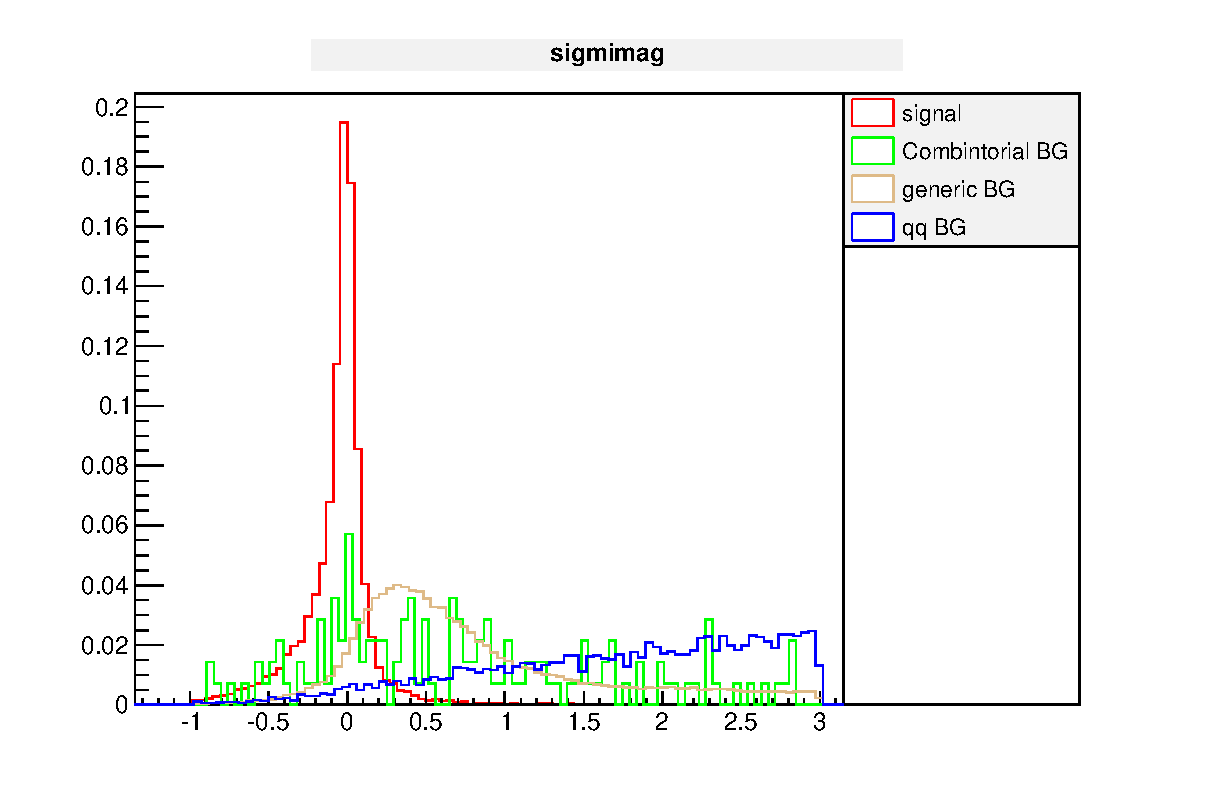
\includegraphics[width=0.3\textwidth]{Controlsample_figure/sigmimag_1223_1.eps}
		\label{simimagdkpi}
	}
		\subfigure[$B^+ \rightarrow D^{0}(K 3 \pi) \ell \nu$]{
		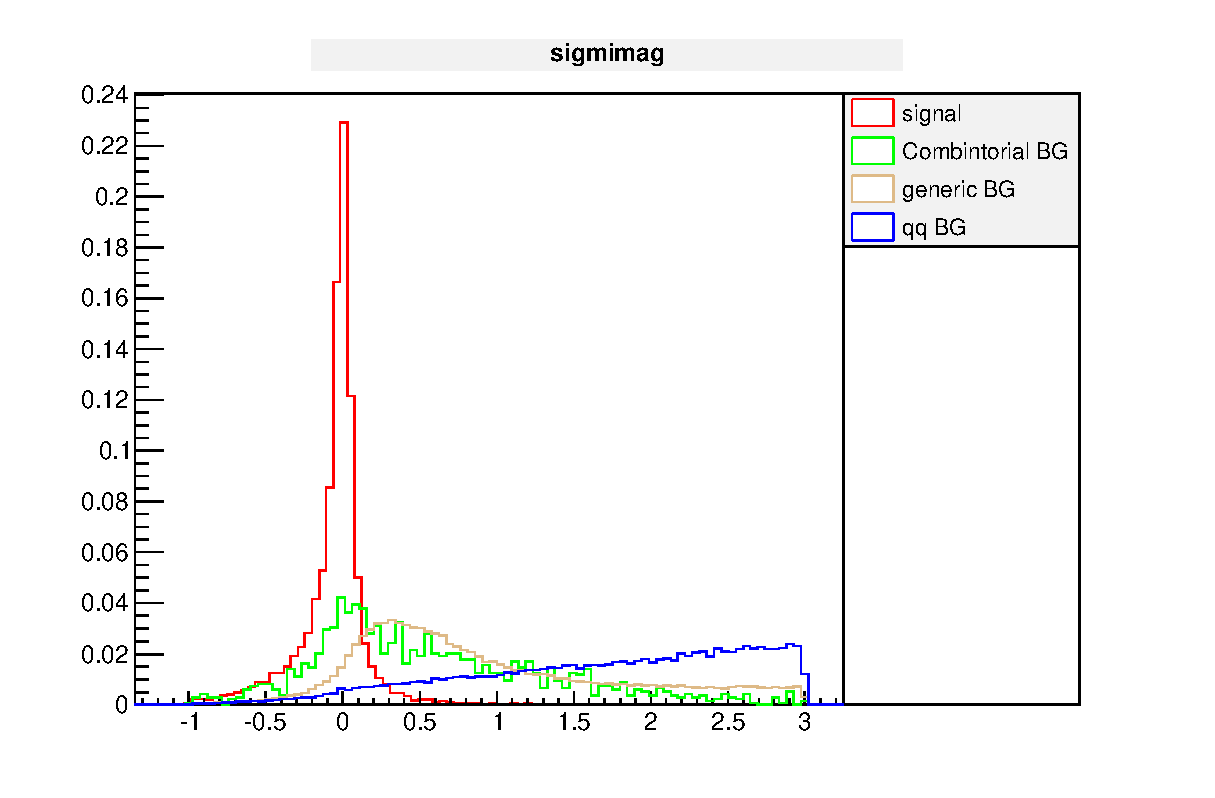
\includegraphics[width=0.3\textwidth]{Controlsample_figure/sigmimag_1223_2.eps}
		\label{simimagdk3pi}
	}
    	\subfigure[$B^+ \rightarrow D^{0}(K_s 2 \pi) \ell \nu$]{
		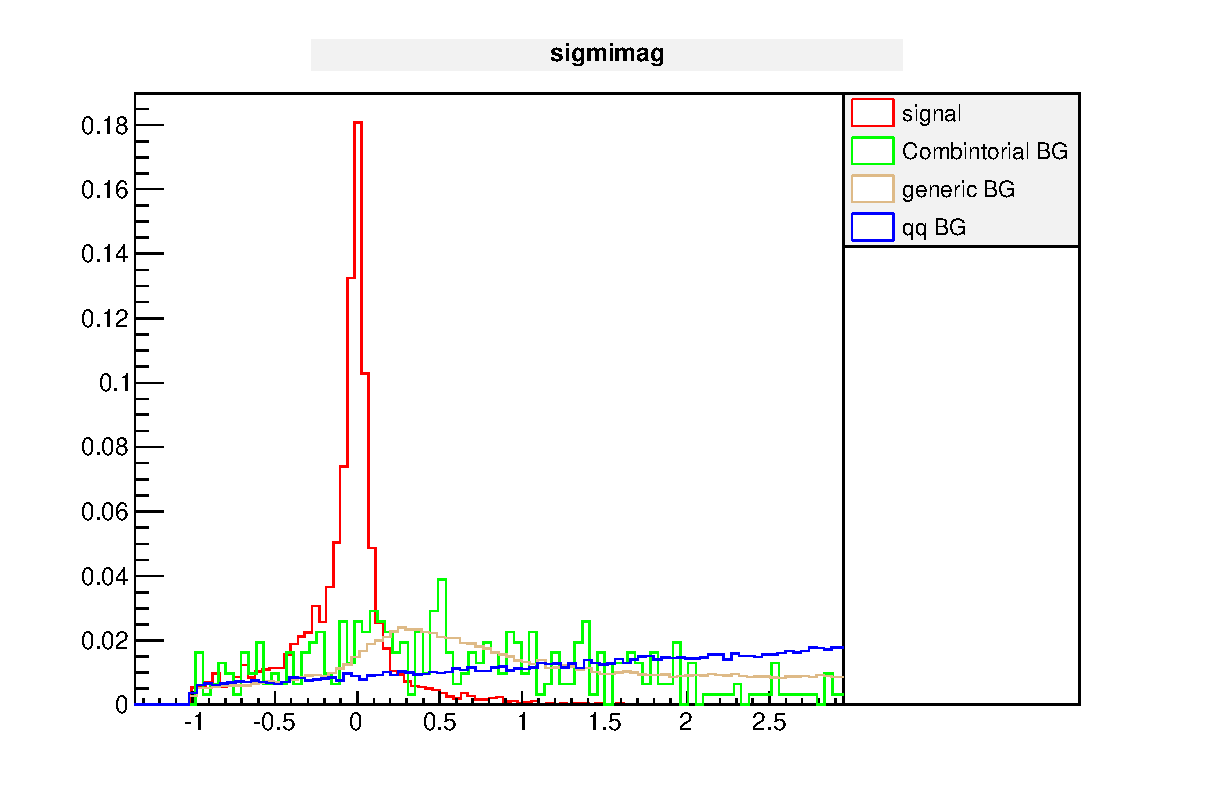
\includegraphics[width=0.3\textwidth]{Controlsample_figure/sigmimag_1223_3.eps}
		\label{simimagdks2pi}
	}
    	\subfigure[$B^+ \rightarrow D^{*0}(K \pi) \ell \nu$]{
		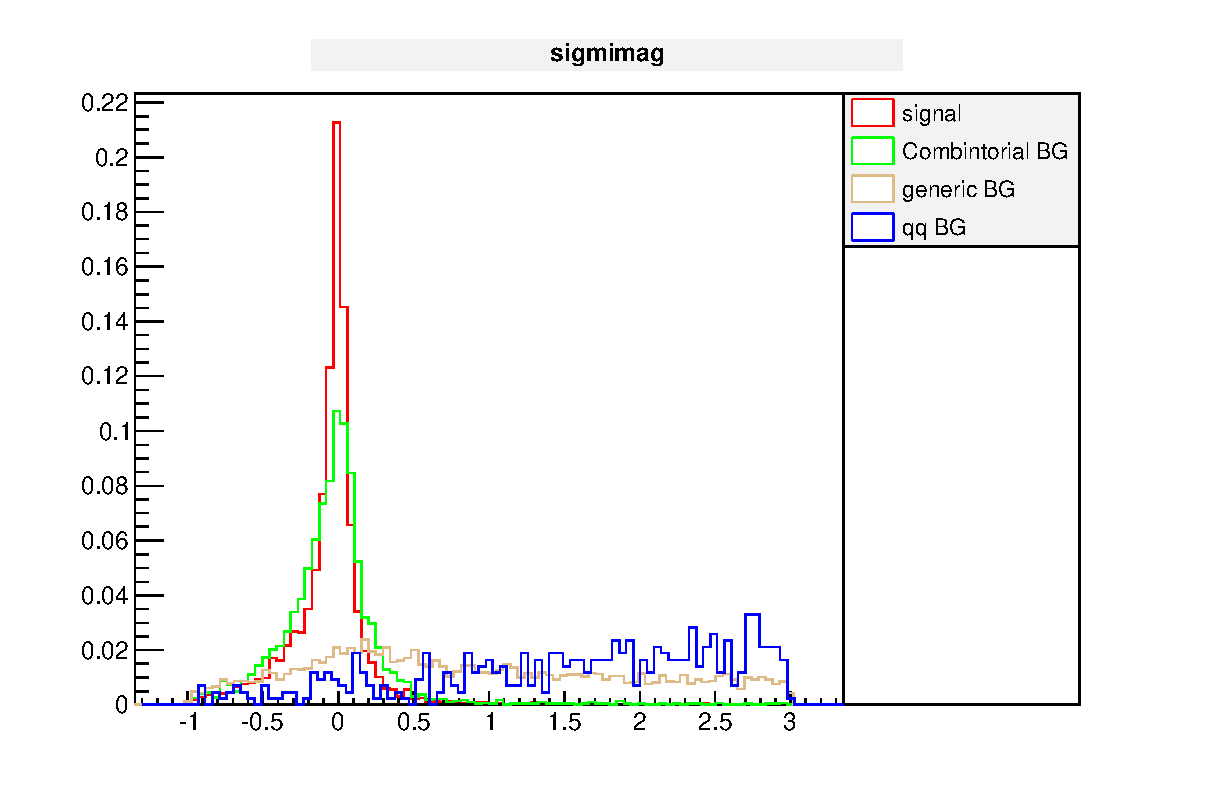
\includegraphics[width=0.3\textwidth]{Controlsample_figure/sigmimag_1223_4.eps}
		\label{simimagdskpi}
	}
    	\subfigure[$B^+ \rightarrow D^{*0}(K 3 \pi) \ell \nu$]{
		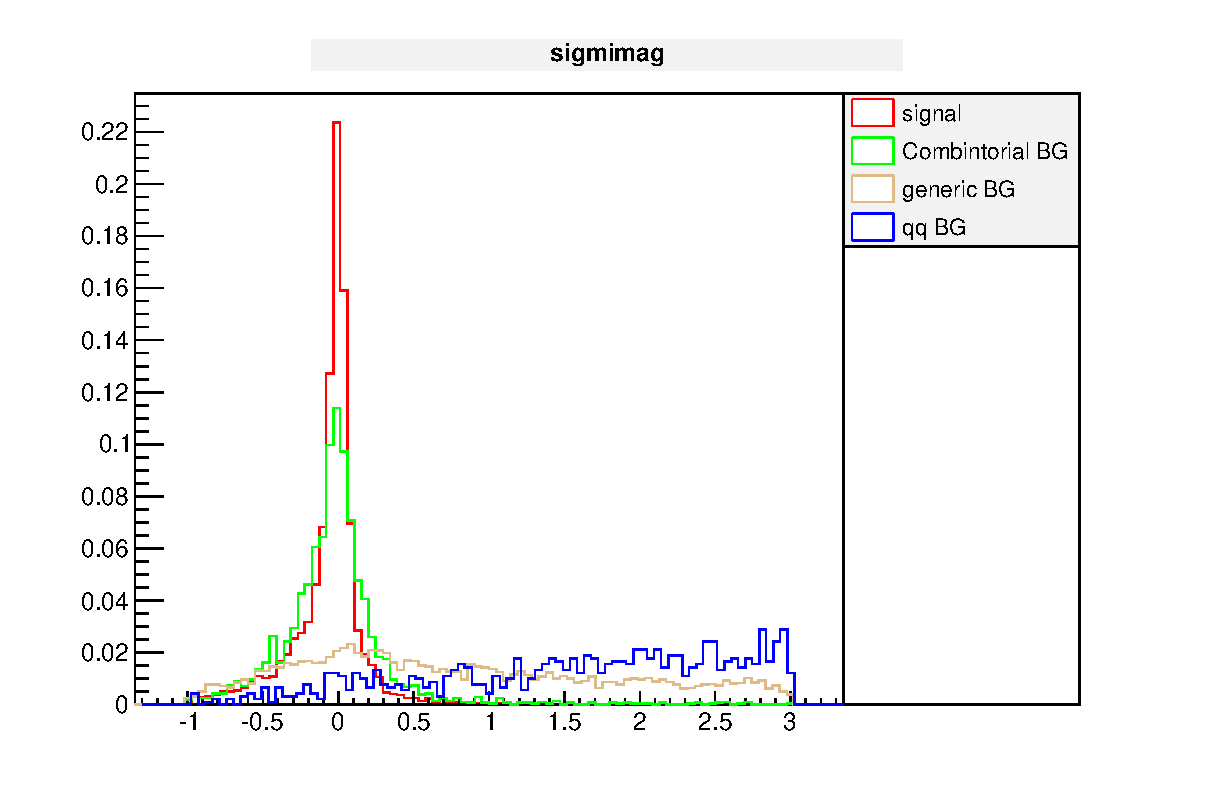
\includegraphics[width=0.3\textwidth]{Controlsample_figure/sigmimag_1223_5.eps}
		\label{simimagdsk3pi}
	}
    	\subfigure[$B^+ \rightarrow D^{*0}(K_s 2 \pi) \ell \nu$]{
		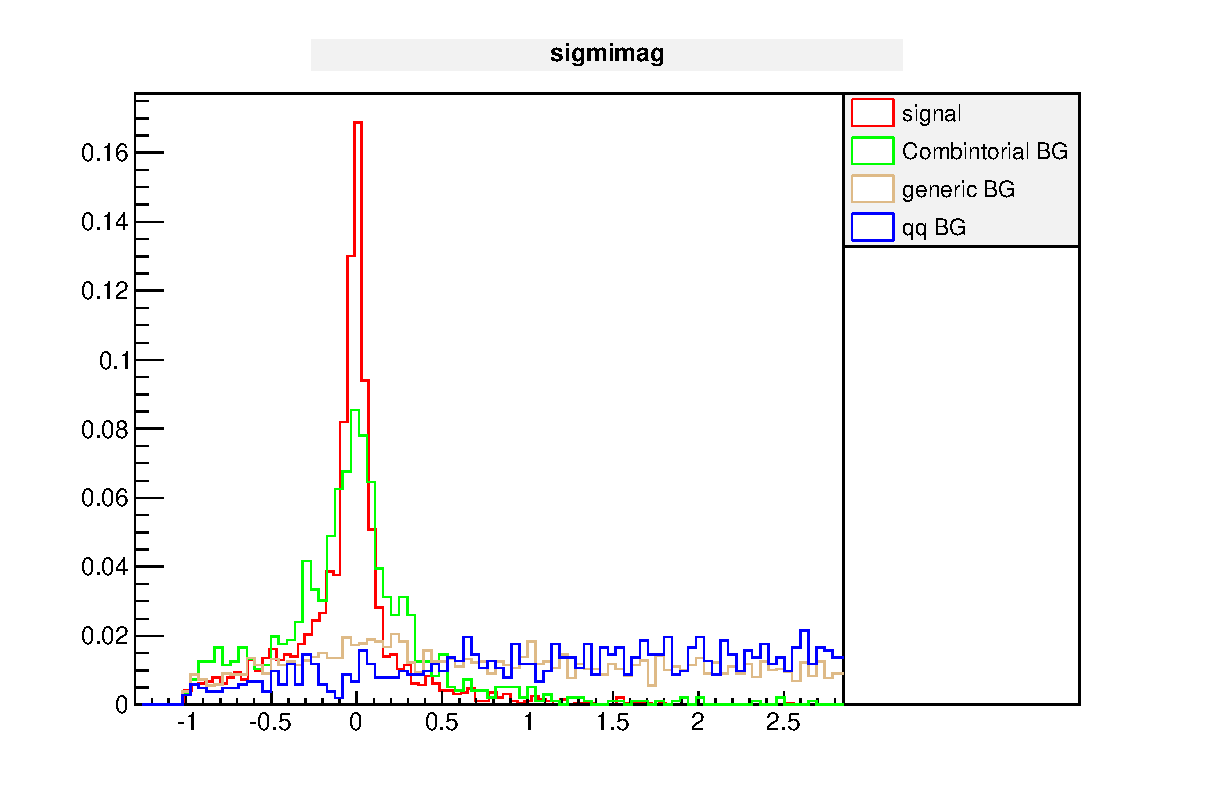
\includegraphics[width=0.3\textwidth]{Controlsample_figure/sigmimag_1223_6.eps}
		\label{simimagdsks2pi}
	}
    	\subfigure[$B^0 \rightarrow D^{-}(K_s \pi) \ell \nu$]{
		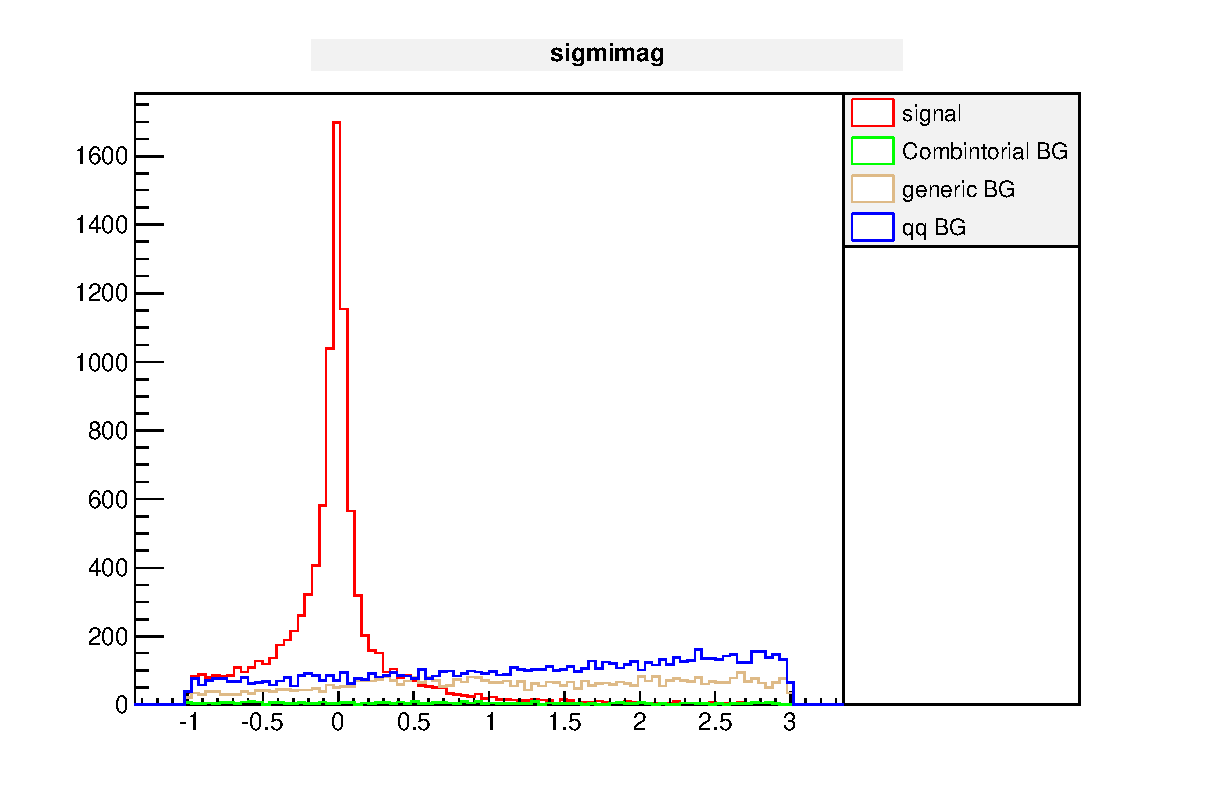
\includegraphics[width=0.45\textwidth]{Controlsample_figure/sigmimag_1025_dmass.eps}
		\label{simimag0dkspi}
	}
    	\subfigure[$B^0 \rightarrow D^{-}(K 2 \pi) \ell \nu$]{
		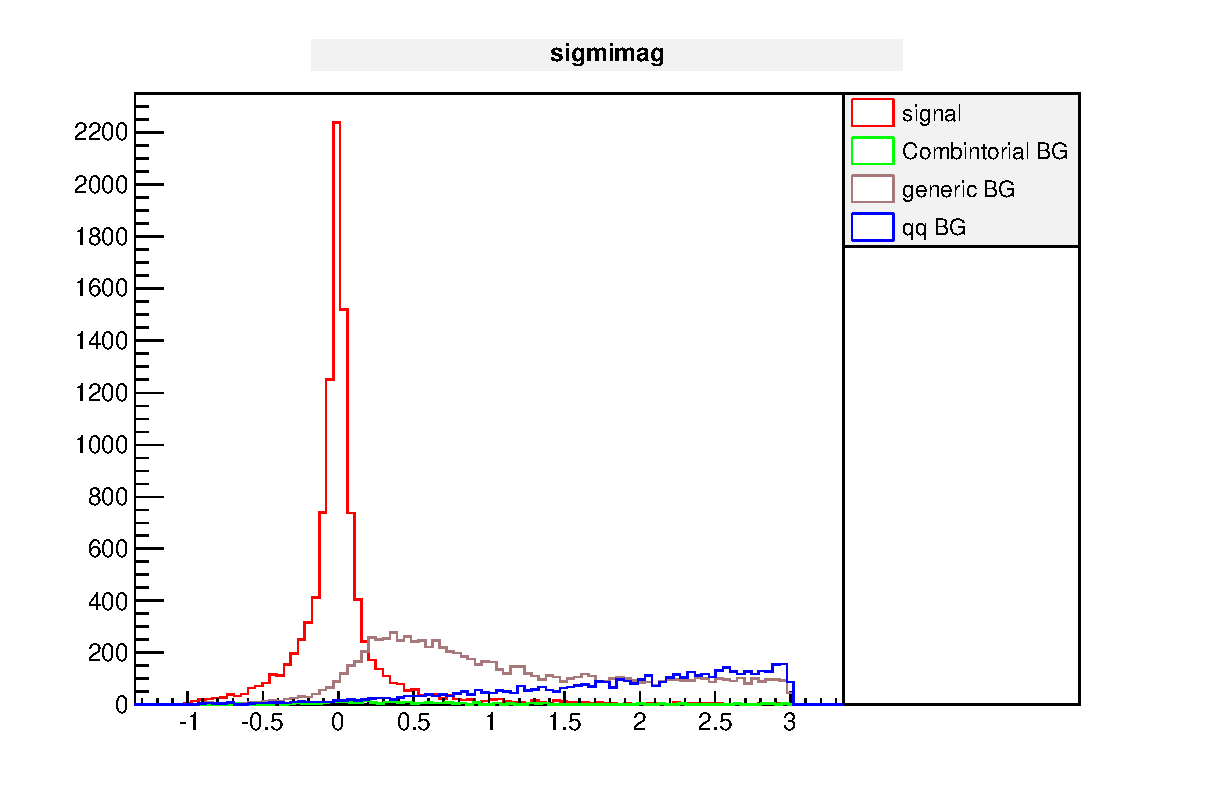
\includegraphics[width=0.45\textwidth]{Controlsample_figure/sigmimag_1025_sigmimag.eps}
		\label{simimag0dk2pi}
	}
	\caption{$m^2_{miss}$ distribution, red represent signal, green represent the combinatorial background,  brown represent the generic background and blue represent continuum background.}
    	\label{sigmimagcon}	
\end{figure}
We set $-1$ > $m^2_{miss}$ > $3$ as the fitting region. For the signal PDF, we use the combination of a Breit-Wigner function and a BifurGauss function. In background PDF, The generic background is modeled by smoothed histogram which is cloned directly from the generic background MC shape, the continuum background is modeled by second order polynomial.PDF modeling with MC sample for all channels are shown in Fig.\ref{sigmimagsigpdf} and Fig. \ref{sigmimagqqpdf}.
\begin{figure}[h]
	\centering
	\subfigure[$B^+ \rightarrow D^{0}(K \pi) \ell \nu$]{
		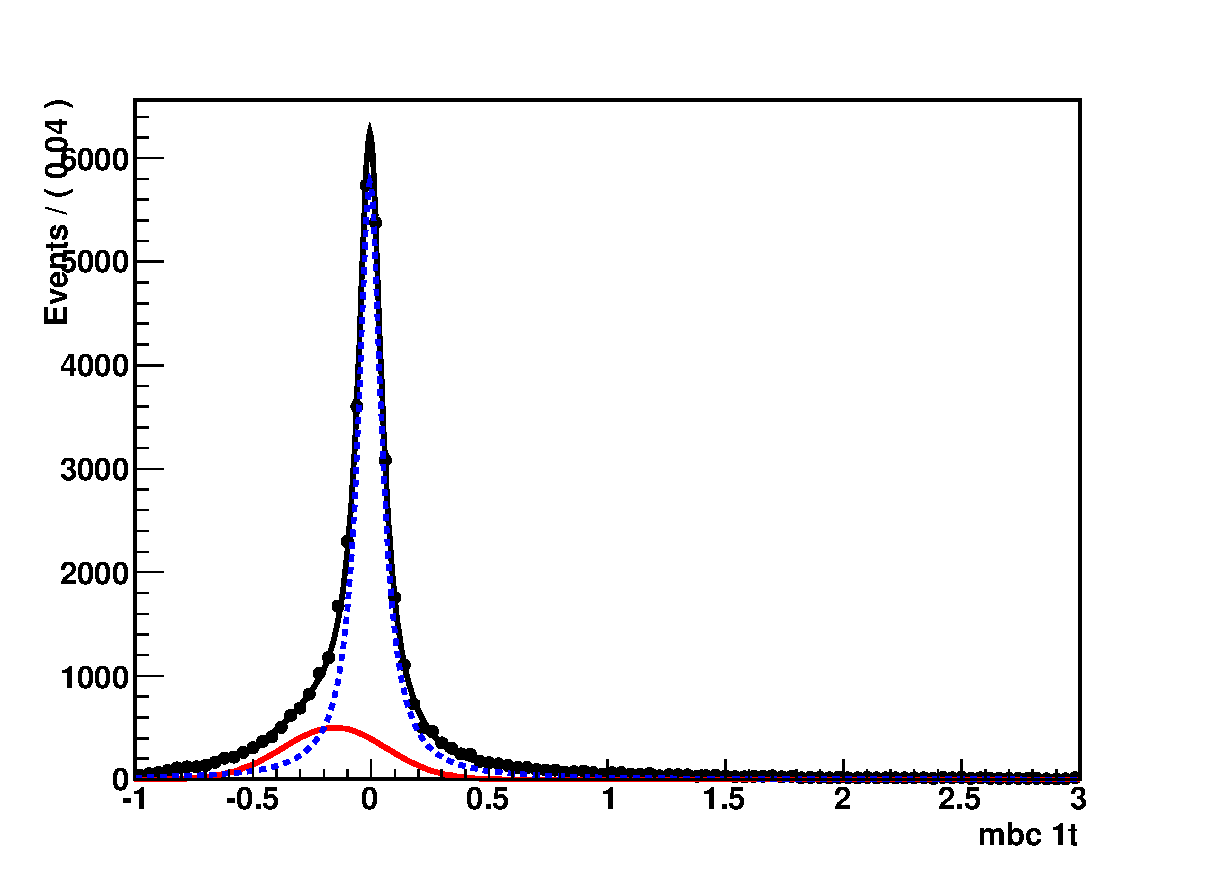
\includegraphics[width=0.3\textwidth]{Controlsample_figure/sigeecl_v2_0428_mbc_1_v2.eps}
		\label{simimagsigpdfdkpi}
	}
		\subfigure[$B^+ \rightarrow D^{0}(K 3 \pi) \ell \nu$]{
		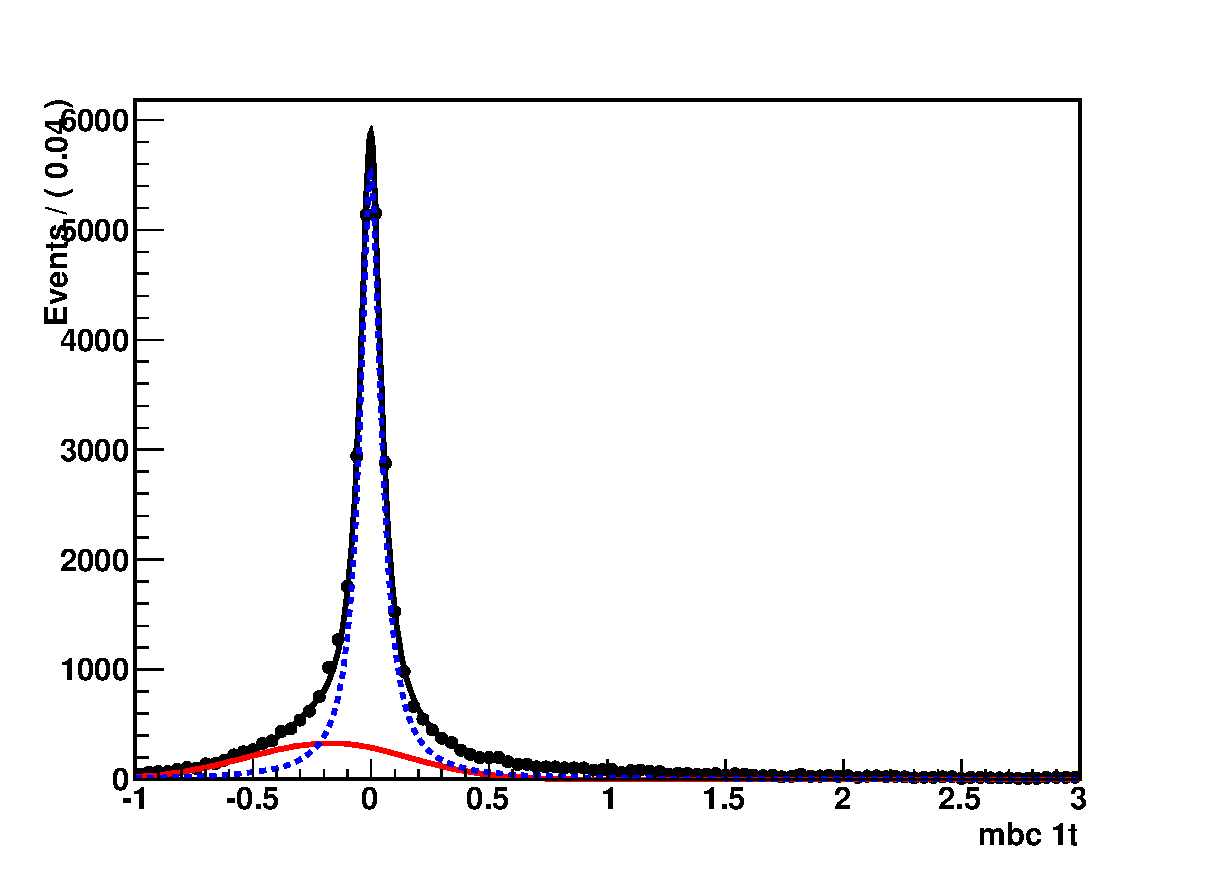
\includegraphics[width=0.3\textwidth]{Controlsample_figure/sigeecl_v2_0428_mbc_2_v2.eps}
		\label{simimagsigpdfdk3pi}
	}
    	\subfigure[$B^+ \rightarrow D^{0}(K_s 2 \pi) \ell \nu$]{
		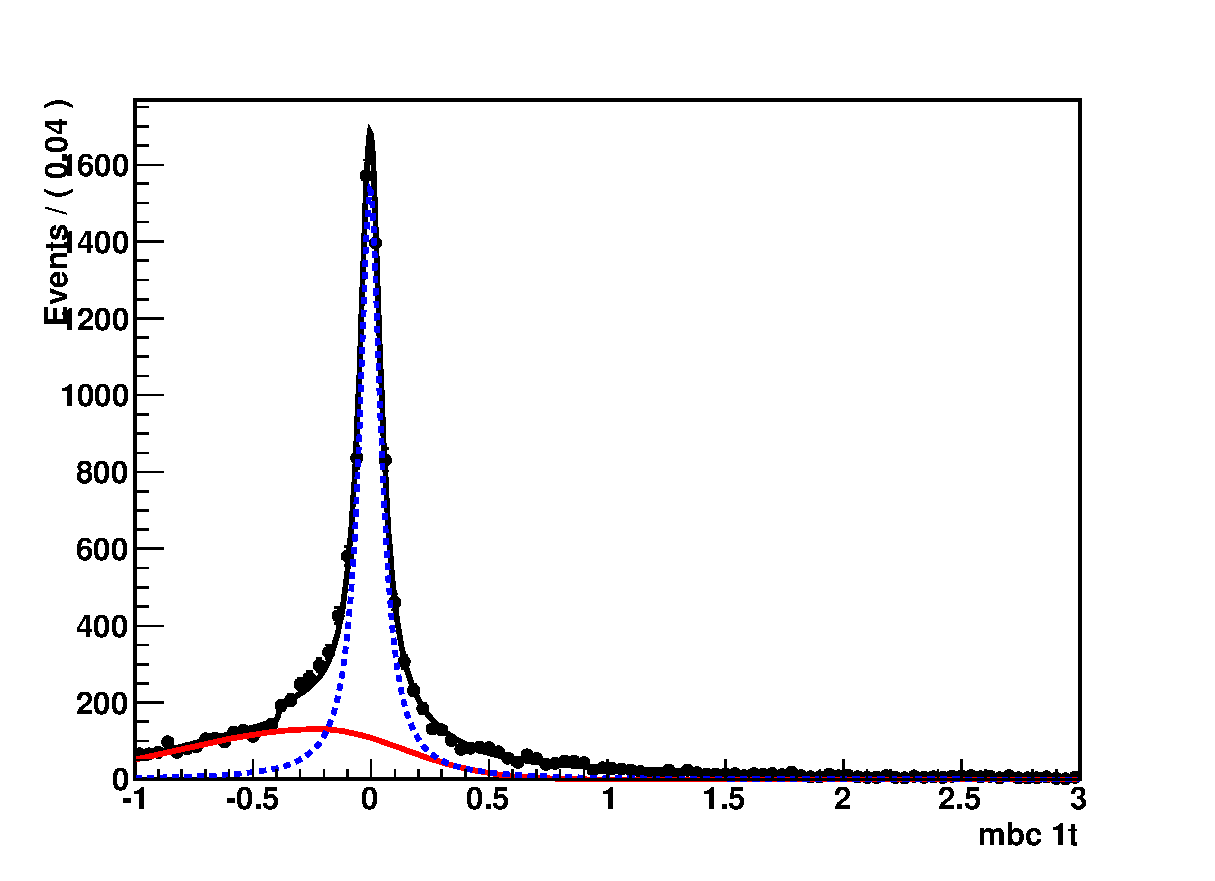
\includegraphics[width=0.3\textwidth]{Controlsample_figure/sigeecl_v2_0428_mbc_3_v2.eps}
		\label{simimagsigpdfdks2pi}
	}
    	\subfigure[$B^+ \rightarrow D^{*0}(K \pi) \ell \nu$]{
		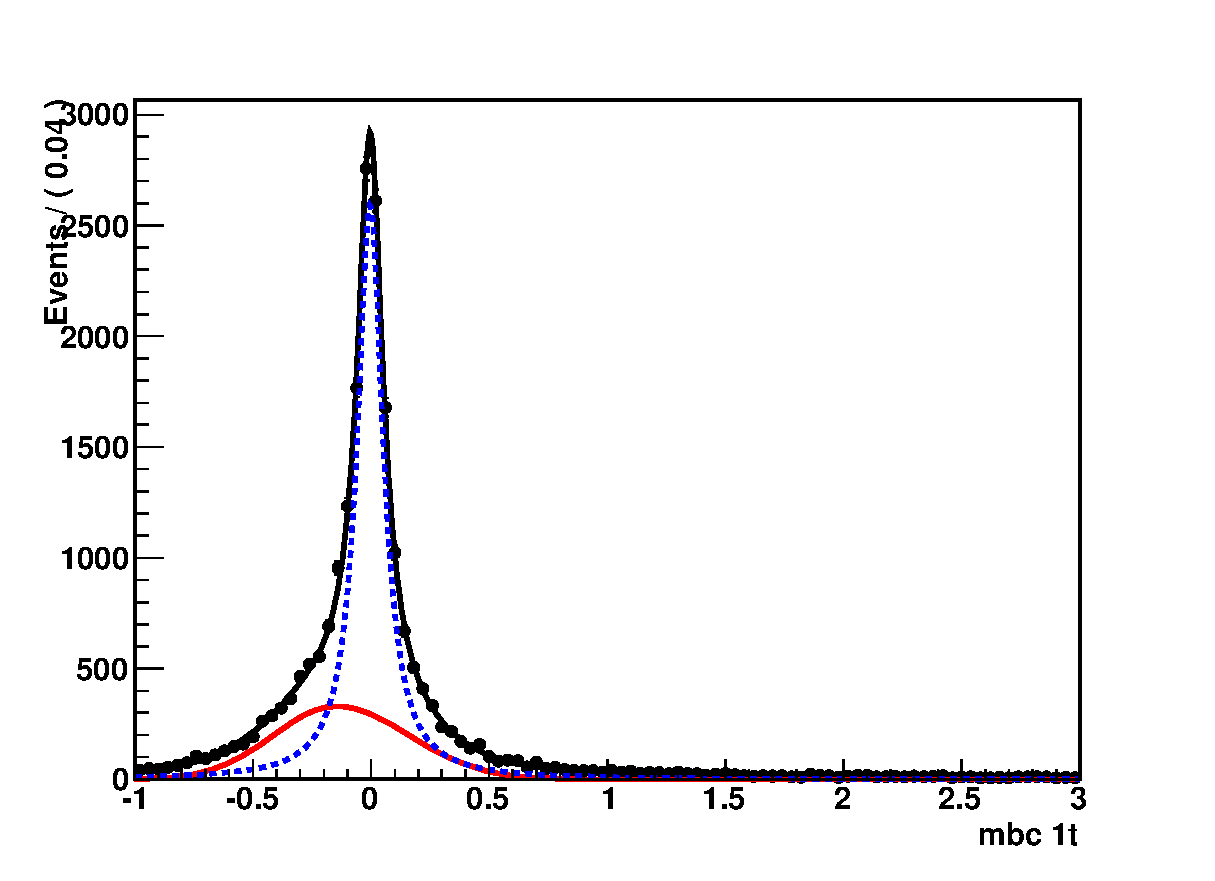
\includegraphics[width=0.3\textwidth]{Controlsample_figure/sigeecl_v2_0428_mbc_4_v2.eps}
		\label{simimagsigpdfdskpi}
	}
    	\subfigure[$B^+ \rightarrow D^{*0}(K 3 \pi) \ell \nu$]{
		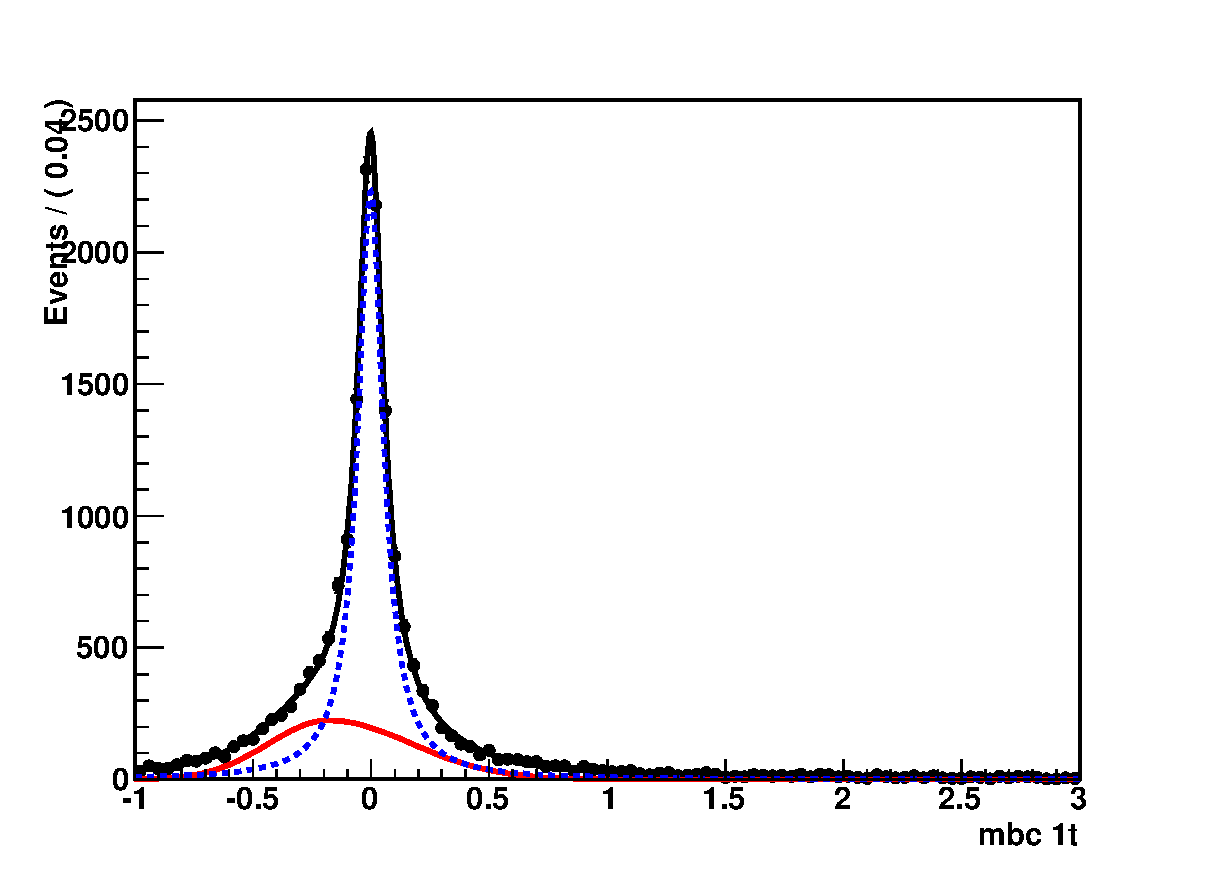
\includegraphics[width=0.3\textwidth]{Controlsample_figure/sigeecl_v2_0428_mbc_5_v2.eps}
		\label{simimagsigpdfdsk3pi}
	}
    	\subfigure[$B^+ \rightarrow D^{*0}(K_s 2 \pi) \ell \nu$]{
		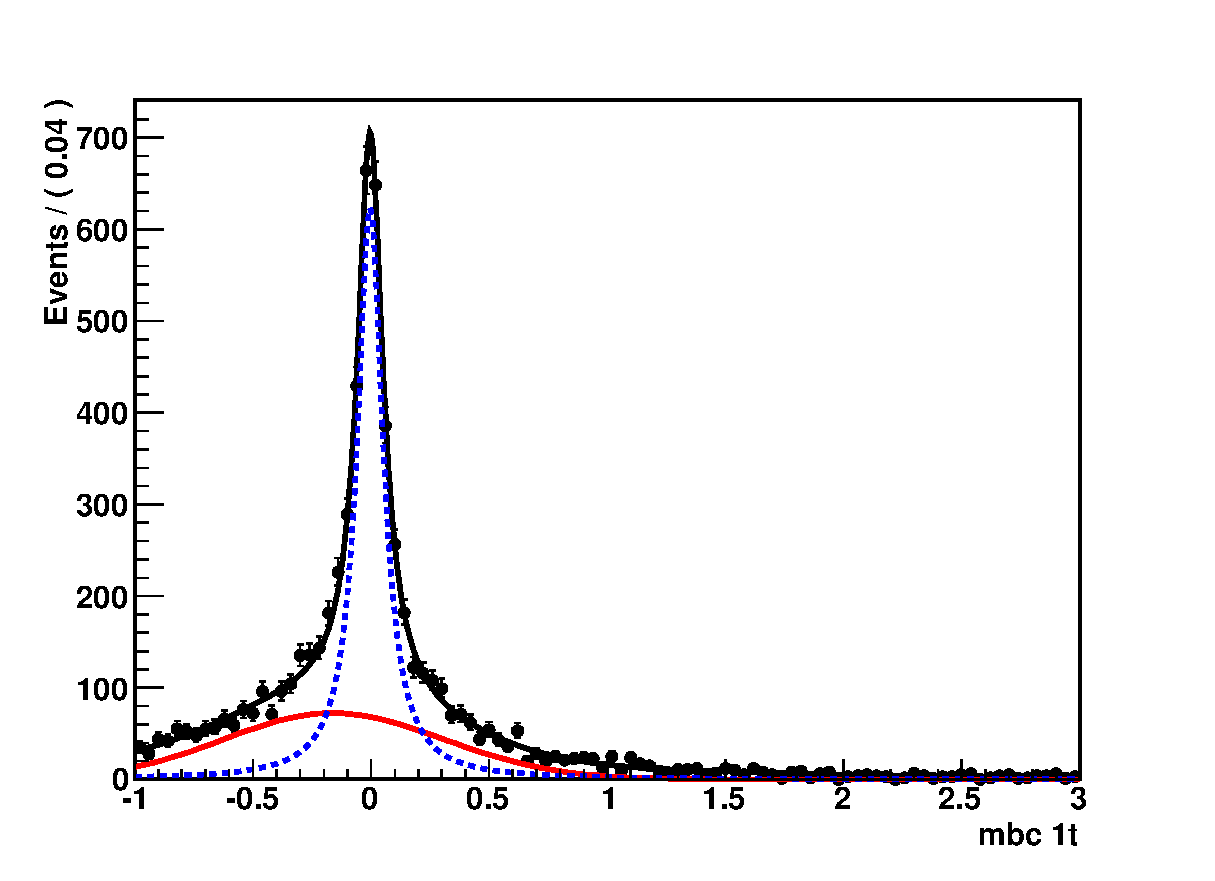
\includegraphics[width=0.3\textwidth]{Controlsample_figure/sigeecl_v2_0428_mbc_6_v2.eps}
		\label{simimagsigpdfdsks2pi}
	}
    	\subfigure[$B^0 \rightarrow D^{-}(K_s \pi) \ell \nu$]{
		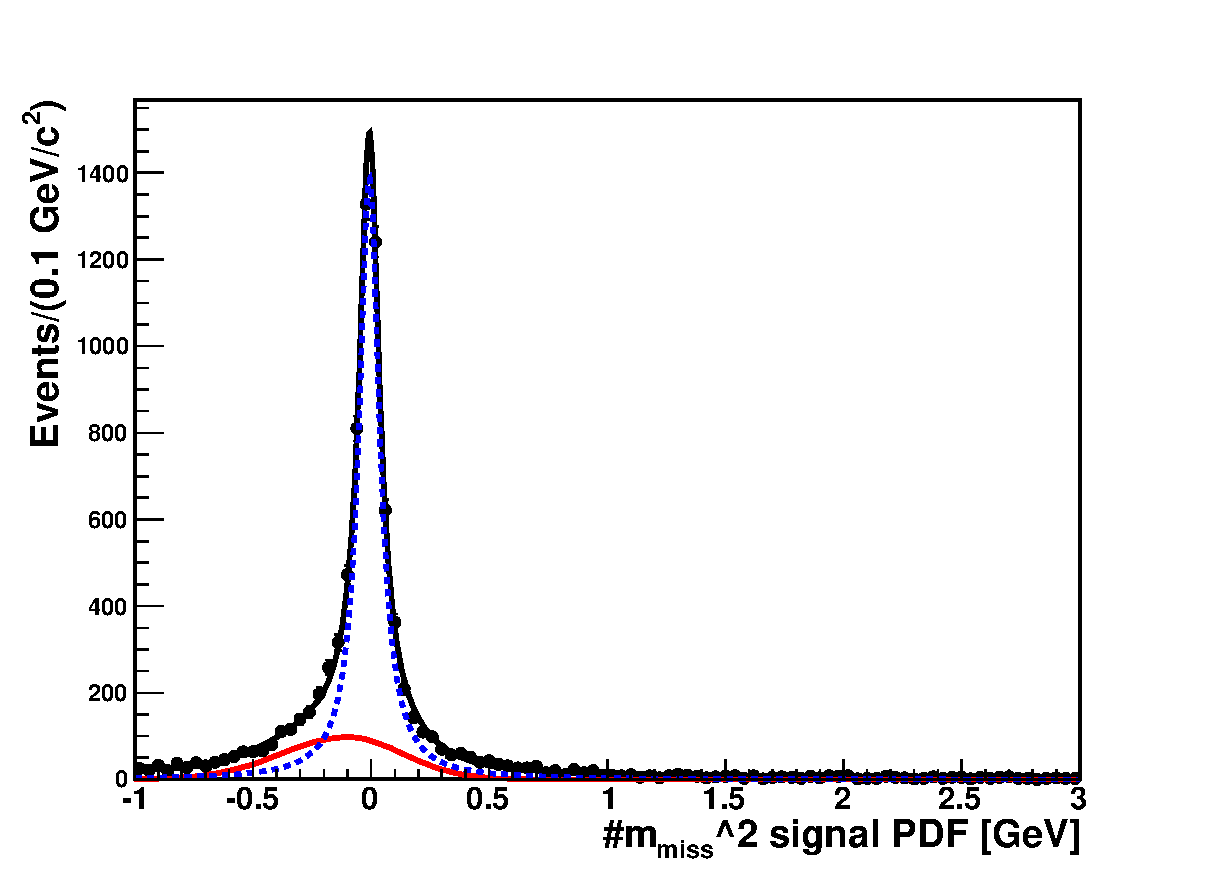
\includegraphics[width=0.45\textwidth]{Controlsample_figure/missingmass_sig_test.eps}
		\label{simimagsigpdf0dkspi}
	}
    	\subfigure[$B^0 \rightarrow D^{-}(K 2 \pi) \ell \nu$]{
		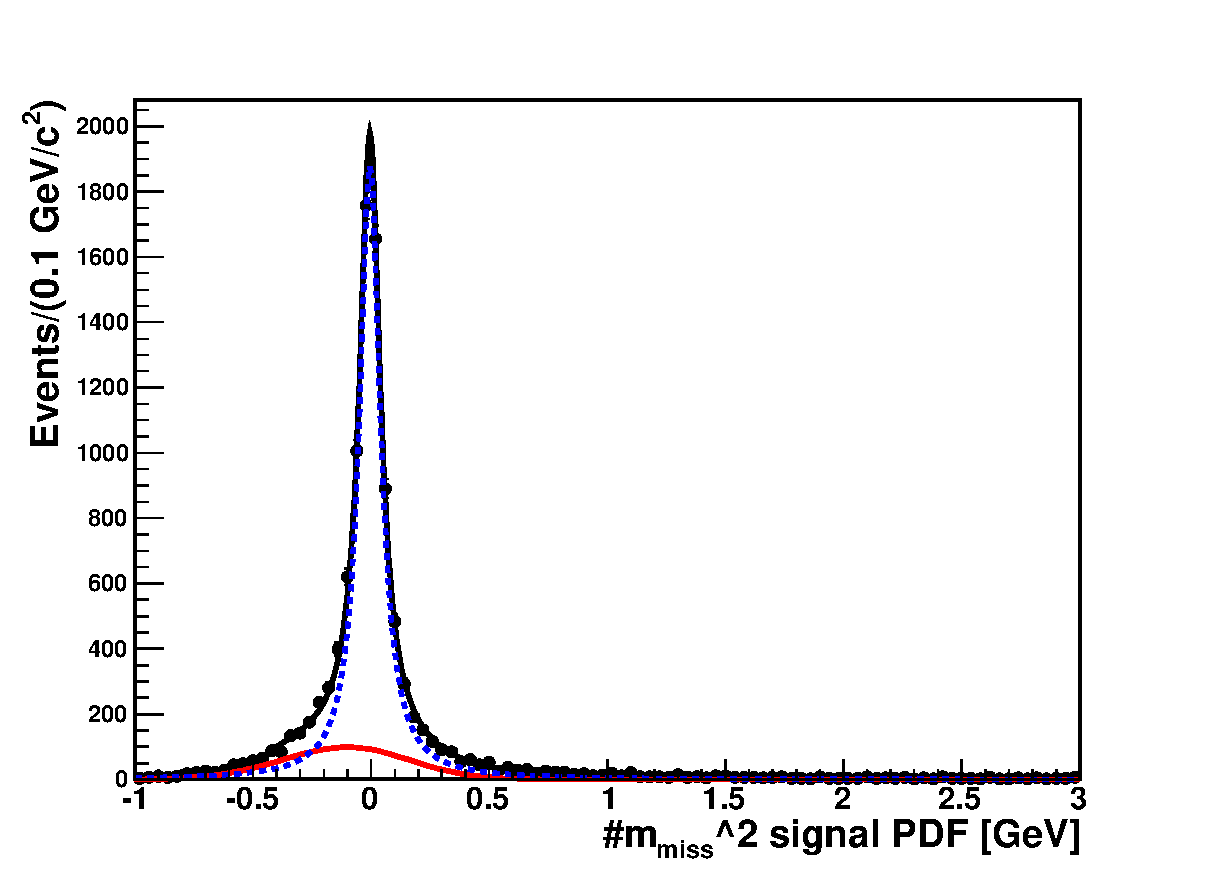
\includegraphics[width=0.45\textwidth]{Controlsample_figure/missingmass_sig_testkpipi.eps}
		\label{simimagsigpdf0dk2pi}
	}
	\caption{Signal PDF.}
    	\label{sigmimagsigpdf}	
\end{figure}
\begin{figure}[h]
	\centering
	\subfigure[$B^+ \rightarrow D^{0}(K \pi) \ell \nu$]{
		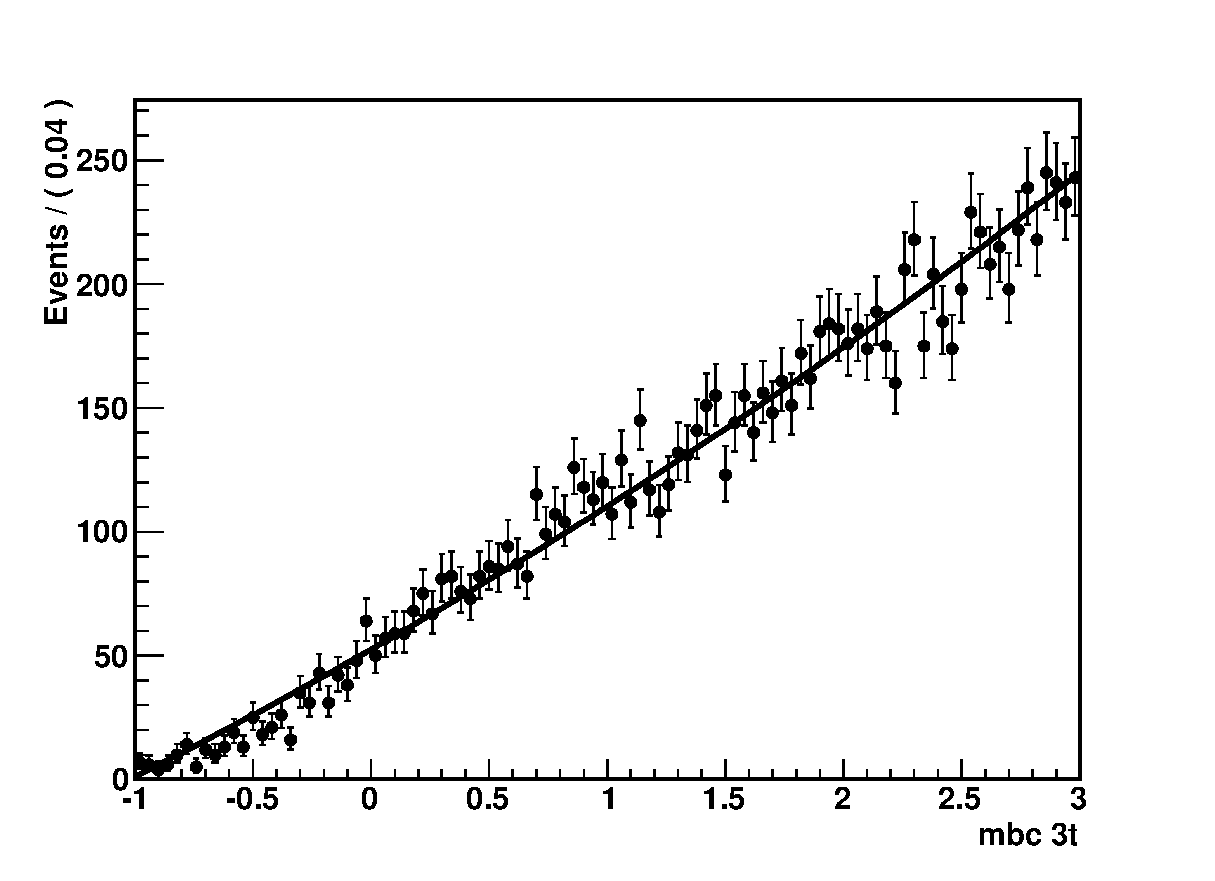
\includegraphics[width=0.3\textwidth]{Controlsample_figure/t1eecl_v2_0428_mbc_1_v2.eps}
		\label{simimagqqpdfdkpi}
	}
		\subfigure[$B^+ \rightarrow D^{0}(K 3 \pi) \ell \nu$]{
		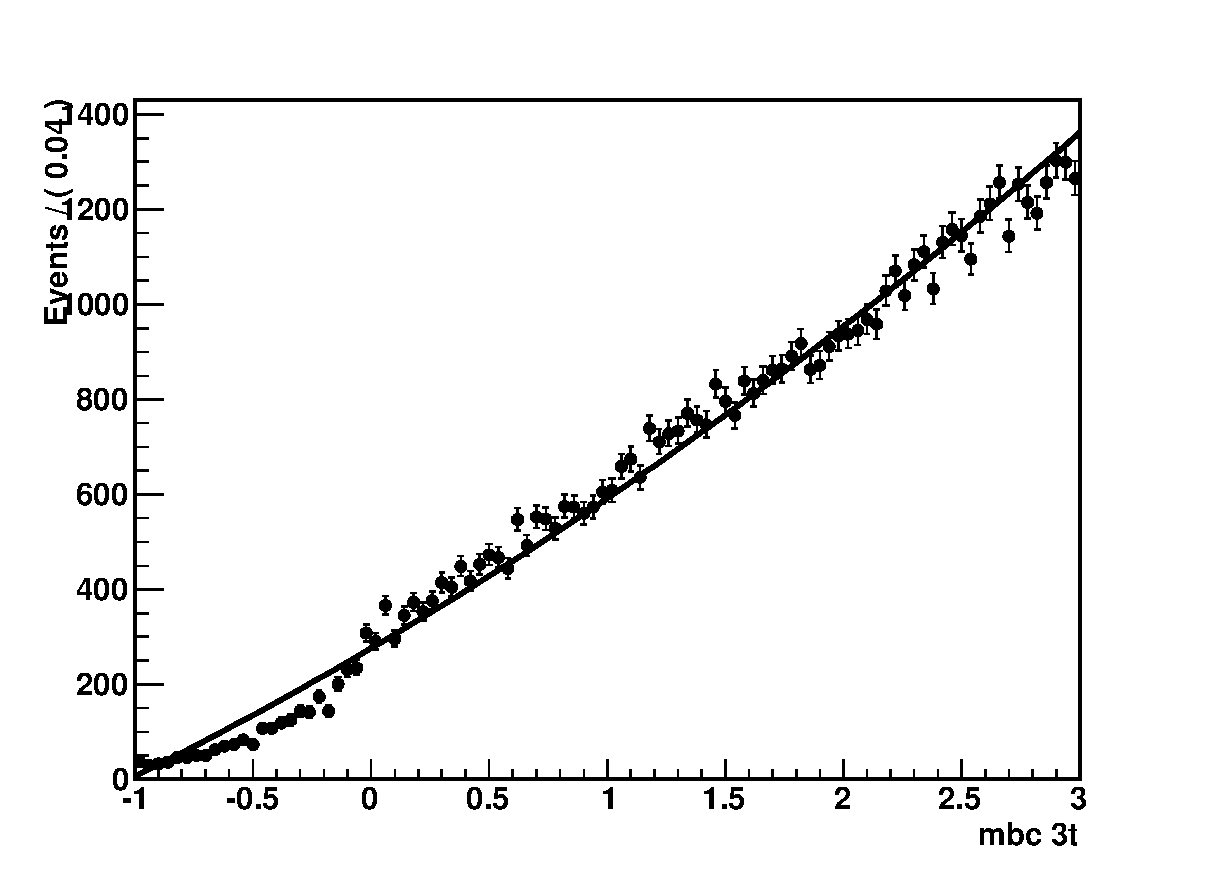
\includegraphics[width=0.3\textwidth]{Controlsample_figure/t1eecl_v2_0428_mbc_2_v2.eps}
		\label{simimagqqpdfdk3pi}
	}
    	\subfigure[$B^+ \rightarrow D^{0}(K_s 2 \pi) \ell \nu$]{
		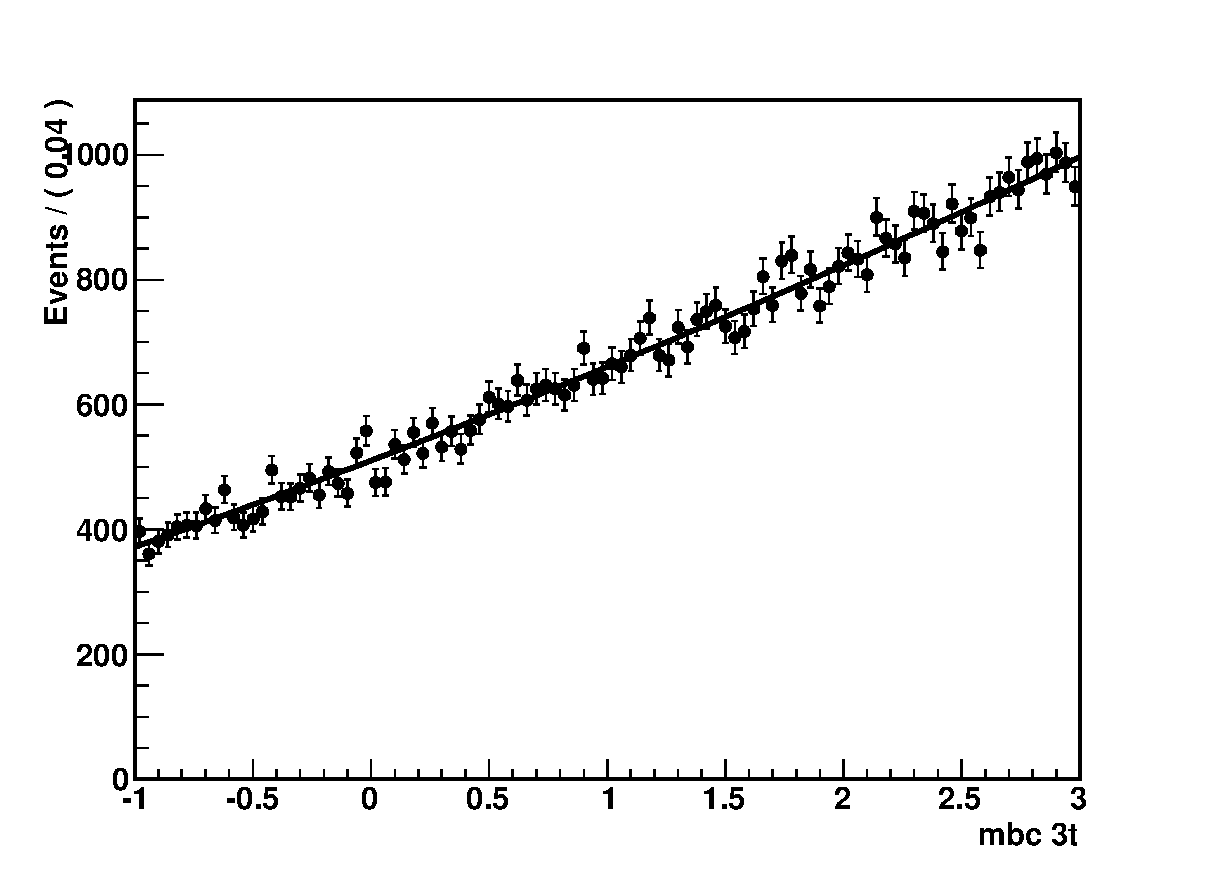
\includegraphics[width=0.3\textwidth]{Controlsample_figure/t1eecl_v2_0428_mbc_3_v2.eps}
		\label{simimagqqpdfdks2pi}
	}
    	\subfigure[$B^+ \rightarrow D^{*0}(K \pi) \ell \nu$]{
		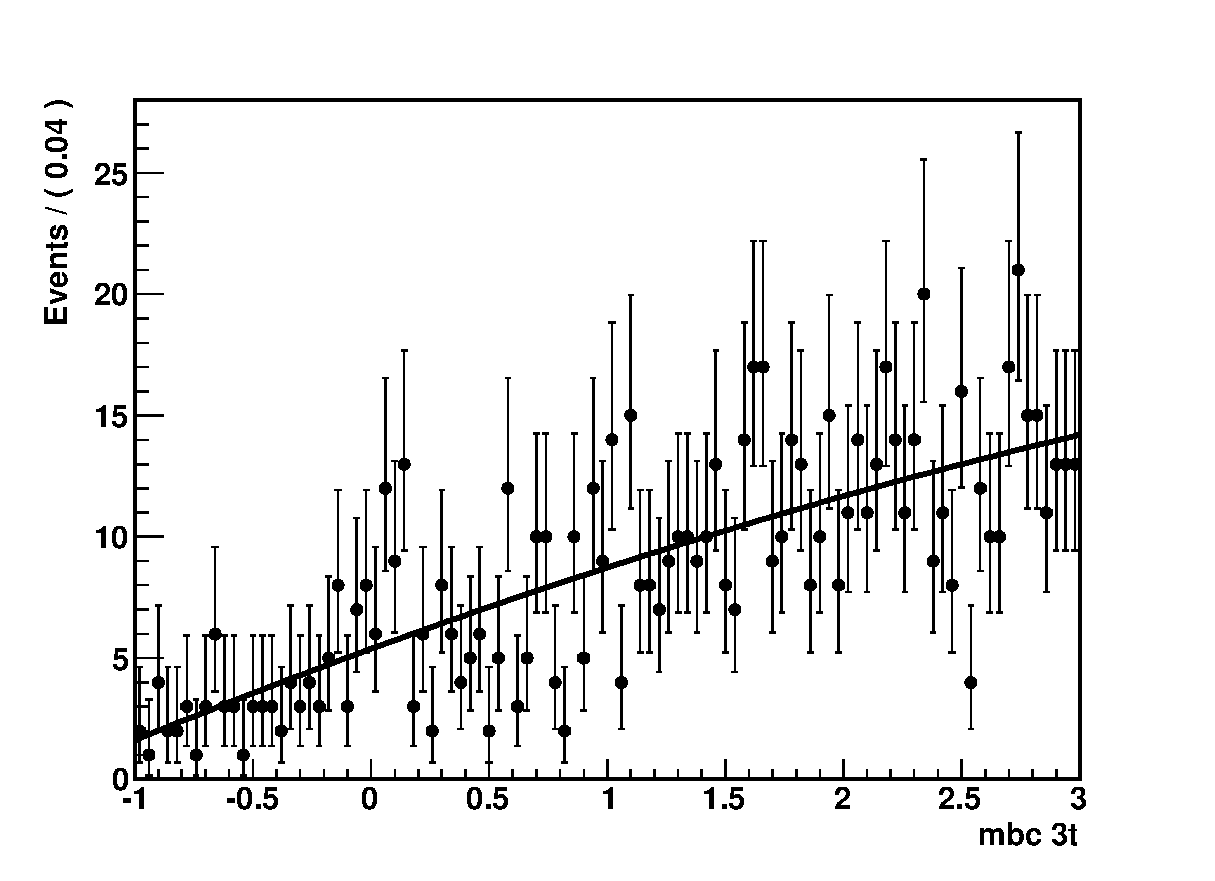
\includegraphics[width=0.3\textwidth]{Controlsample_figure/t1eecl_v2_0428_mbc_4_v2.eps}
		\label{simimagqqpdfdskpi}
	}
    	\subfigure[$B^+ \rightarrow D^{*0}(K 3 \pi) \ell \nu$]{
		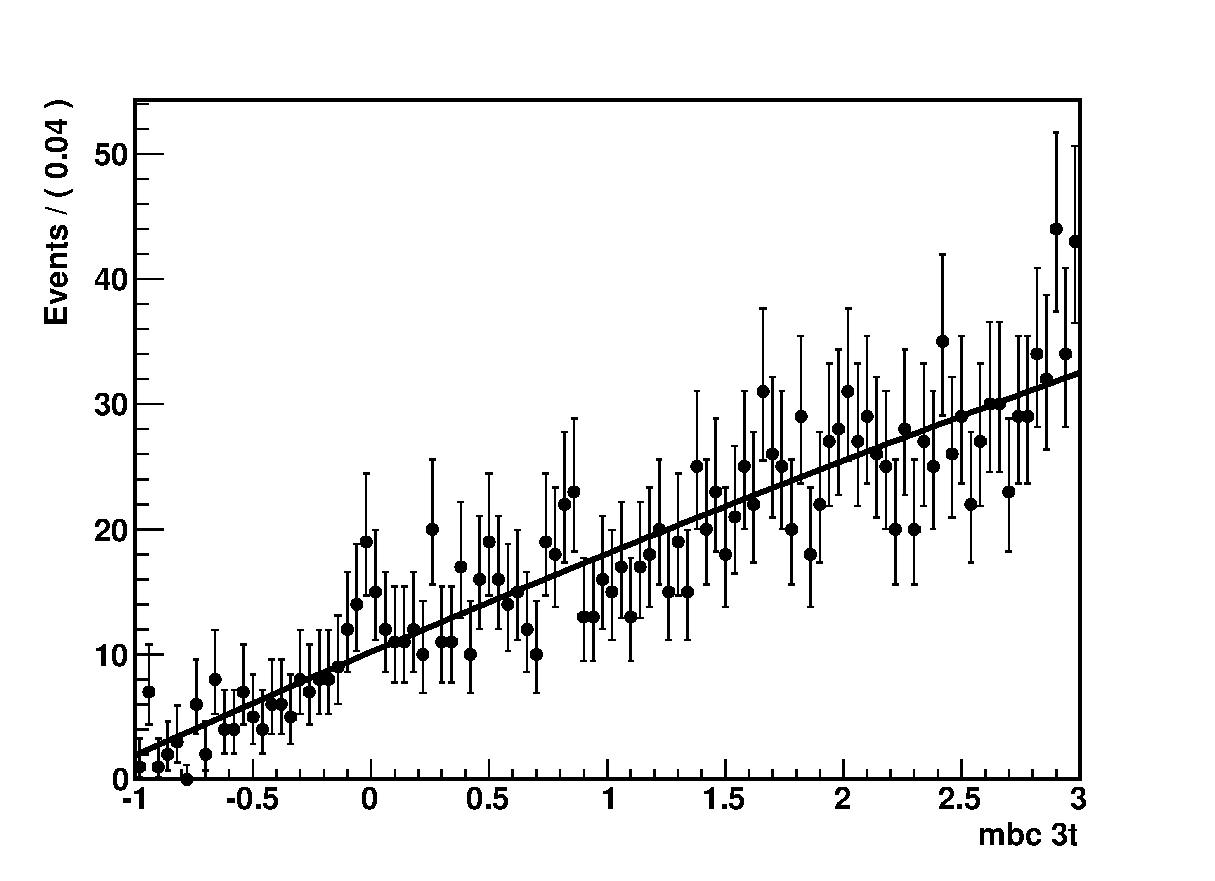
\includegraphics[width=0.3\textwidth]{Controlsample_figure/t1eecl_v2_0428_mbc_5_v2.eps}
		\label{simimagqqpdfdsk3pi}
	}
    	\subfigure[$B^+ \rightarrow D^{*0}(K_s 2 \pi) \ell \nu$]{
		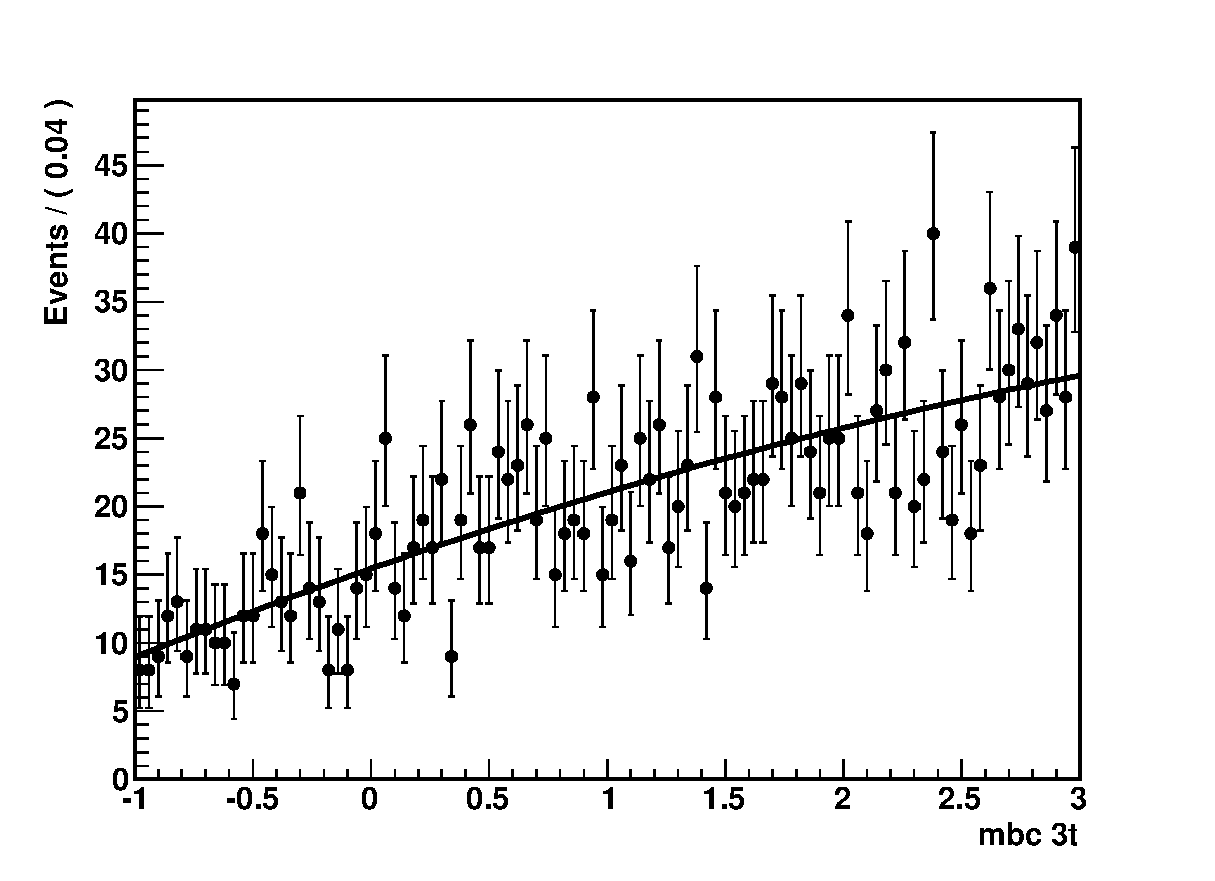
\includegraphics[width=0.3\textwidth]{Controlsample_figure/t1eecl_v2_0428_mbc_6_v2.eps}
		\label{simimagqqpdfdsks2pi}
	}
    	\subfigure[$B^0 \rightarrow D^{-}(K_s \pi) \ell \nu$]{
		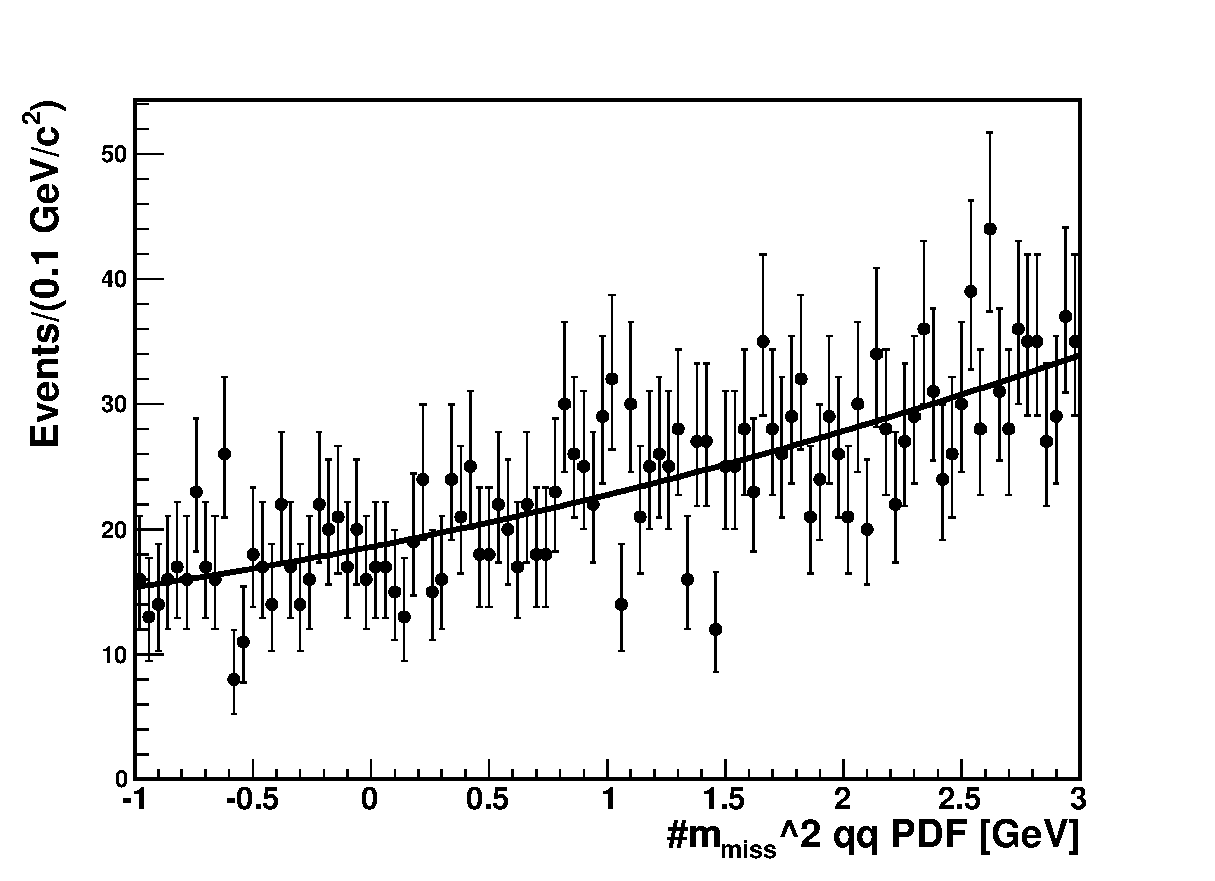
\includegraphics[width=0.45\textwidth]{Controlsample_figure/missingmass_qq_test.eps}
		\label{simimagqqpdf0dkspi}
	}
    	\subfigure[$B^0 \rightarrow D^{-}(K 2 \pi) \ell \nu$]{
		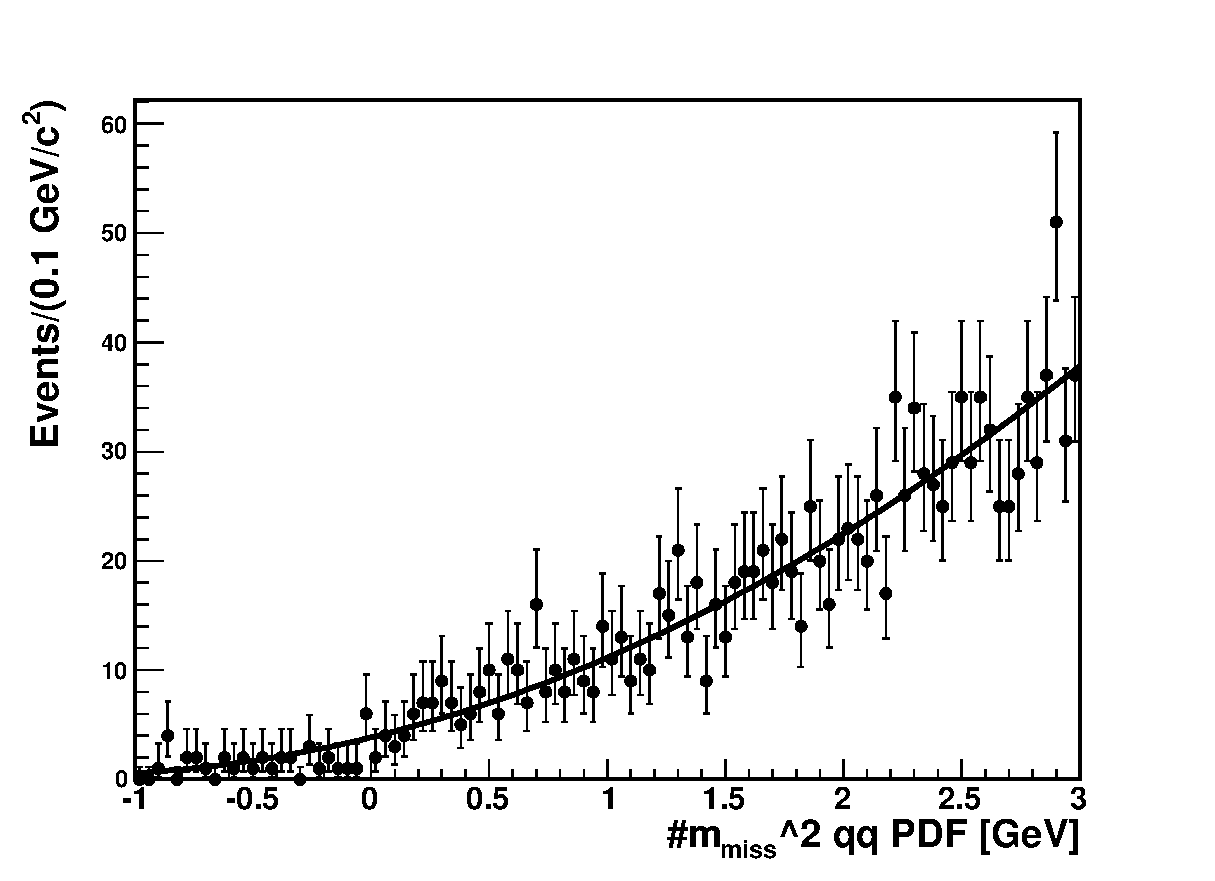
\includegraphics[width=0.45\textwidth]{Controlsample_figure/missingmass_qq_testkpipi.eps}
		\label{simimagqqpdf0dk2pi}
	}
	\caption{Continuum PDF.}
    	\label{sigmimagqqpdf}	
\end{figure}
\clearpage
\section{Measurement}
To avoid the measurement bias, we measure the branching ratio mode-by-mode respectively. In data fitting, the signal, generic and continuum PDF are all fix in order to get the best fitting result. The data fit result are shown in Fig. \ref{condatafit}. The branching ratio measurement result and efficiency are shown in table \ref{t:brbeforec}.   
\begin{figure}[h]
	\centering
	\subfigure[$B^+ \rightarrow D^{0}(K \pi) \ell \nu$]{
		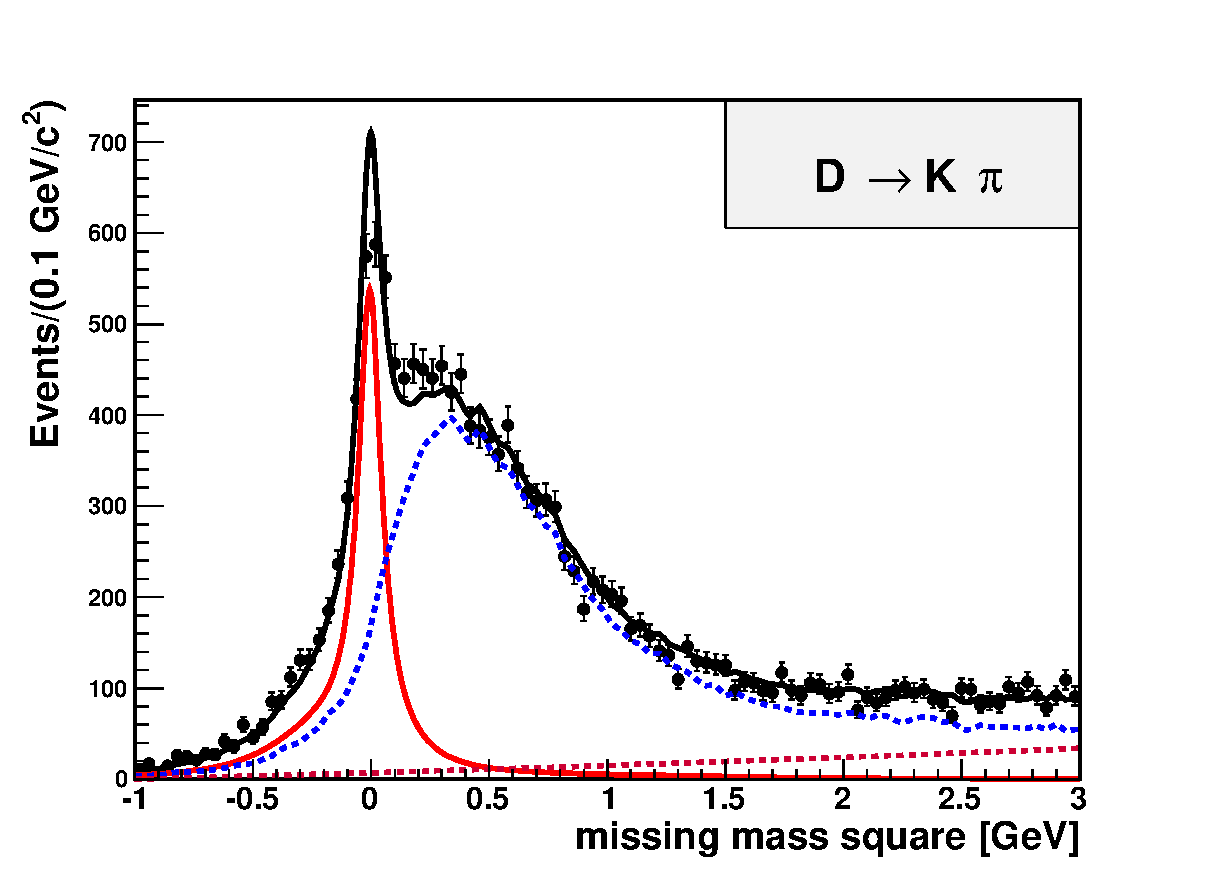
\includegraphics[width=0.3\textwidth]{Controlsample_figure/eecl_v2_0428_mbc_1_v2.eps}
		\label{condatafitdkpi}
	}
		\subfigure[$B^+ \rightarrow D^{0}(K 3 \pi) \ell \nu$]{
		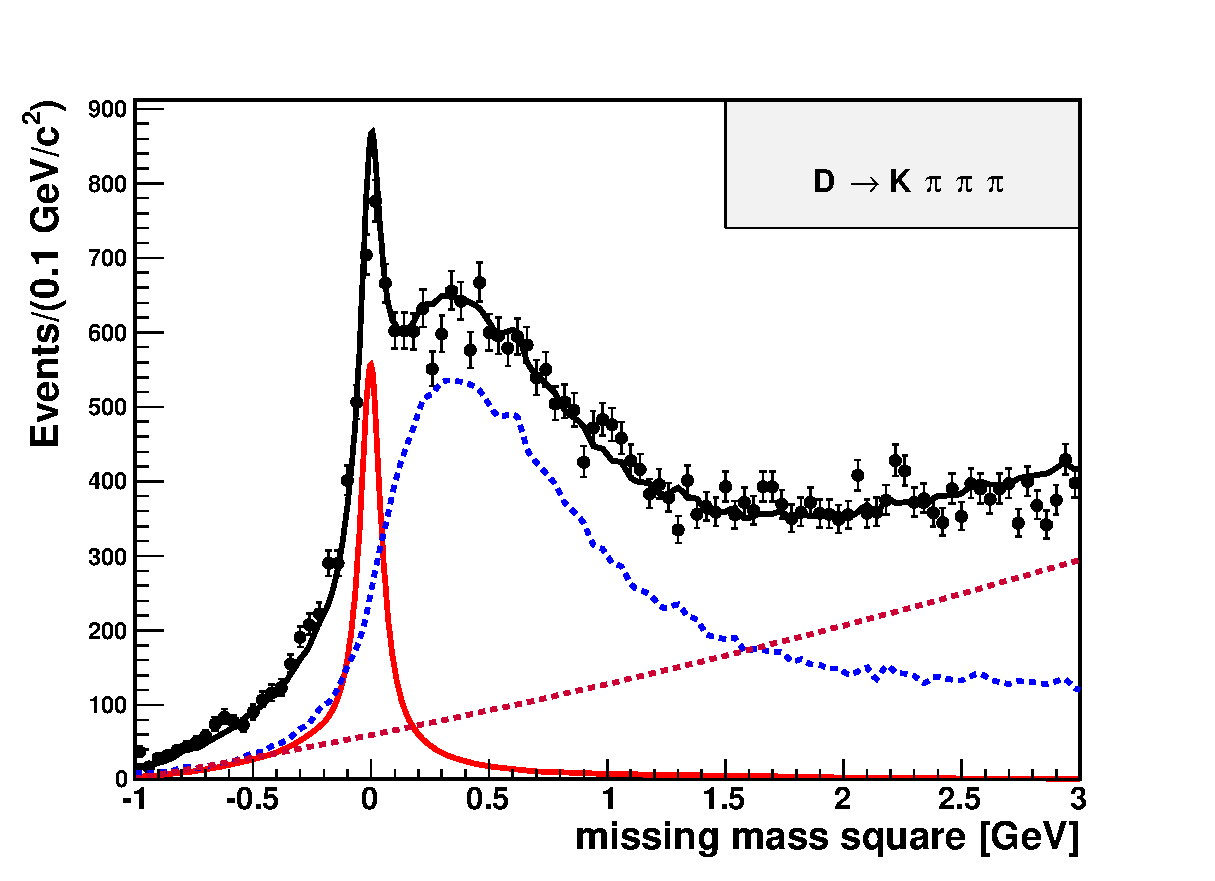
\includegraphics[width=0.3\textwidth]{Controlsample_figure/eecl_v2_0428_mbc_2_v2.eps}
		\label{condatafitdk3pi}
	}
    	\subfigure[$B^+ \rightarrow D^{0}(K_s 2 \pi) \ell \nu$]{
		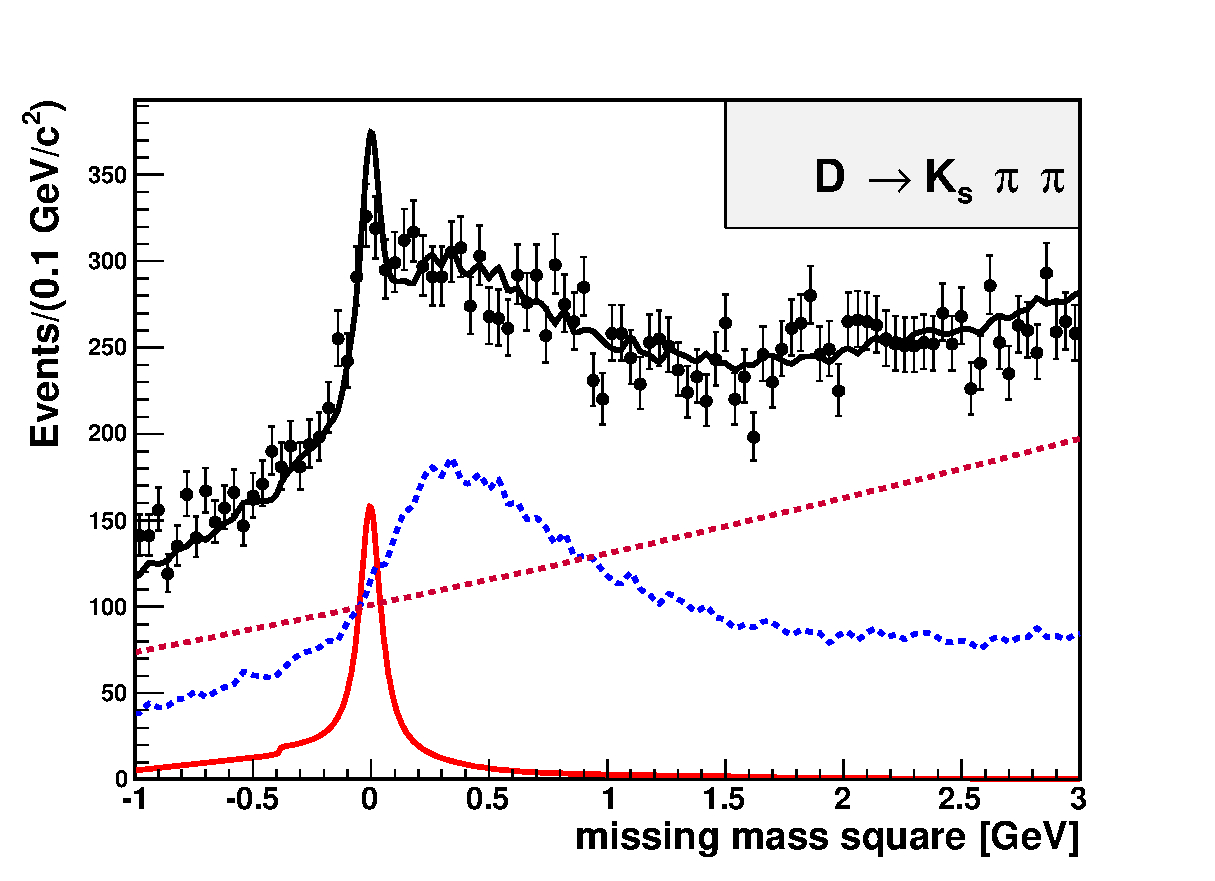
\includegraphics[width=0.3\textwidth]{Controlsample_figure/eecl_v2_0428_mbc_3_v2.eps}
		\label{condatafitdks2pi}
	}
    	\subfigure[$B^+ \rightarrow D^{*0}(K \pi) \ell \nu$]{
		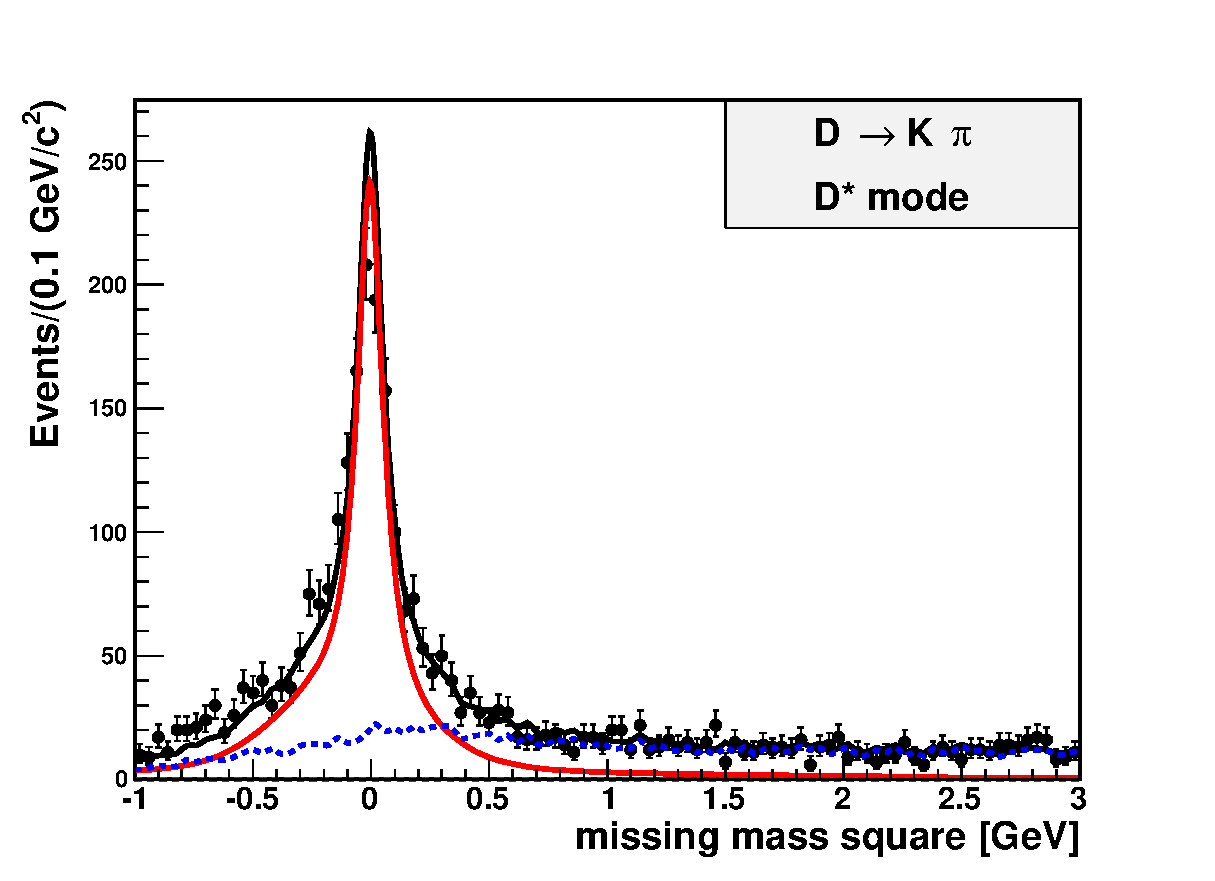
\includegraphics[width=0.3\textwidth]{Controlsample_figure/eecl_v2_0428_mbc_4_v2.eps}
		\label{condatafitdskpi}
	}
    	\subfigure[$B^+ \rightarrow D^{*0}(K 3 \pi) \ell \nu$]{
		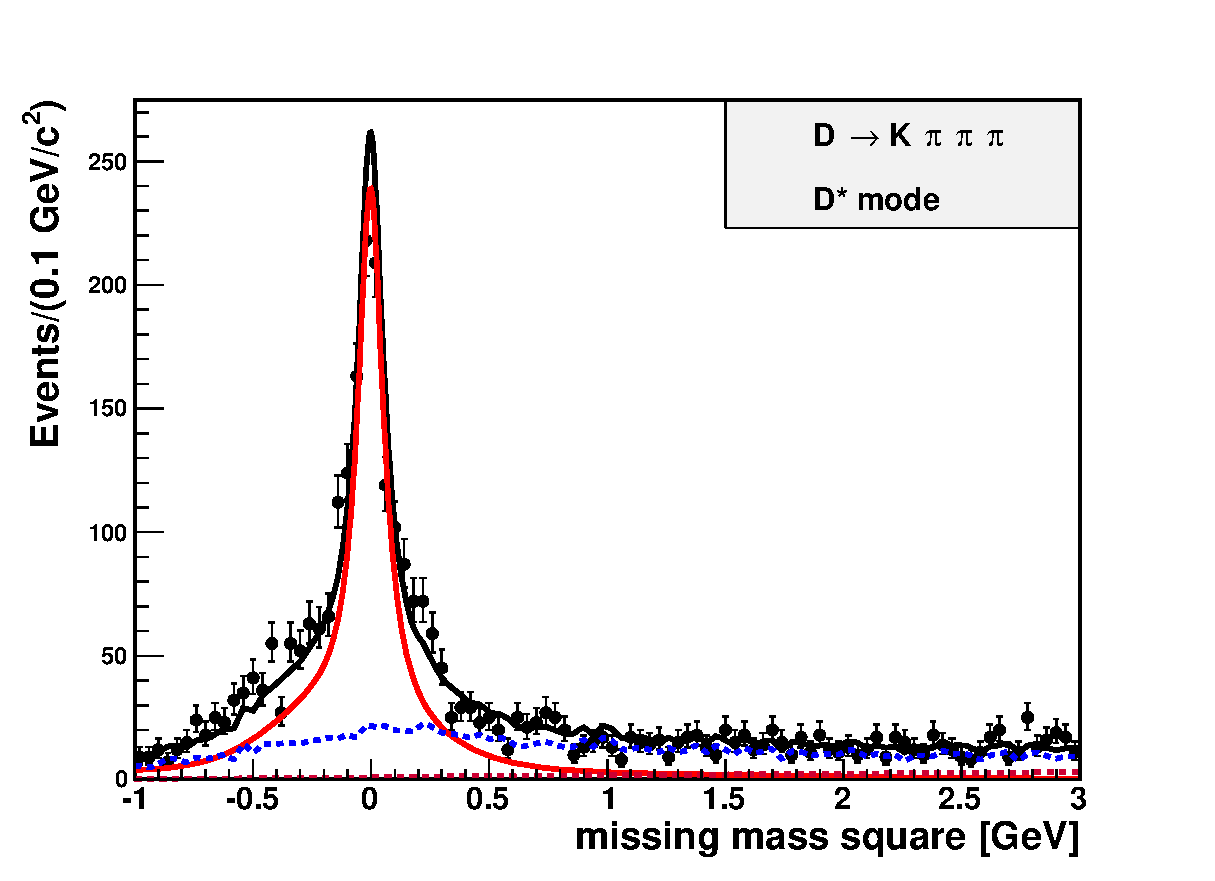
\includegraphics[width=0.3\textwidth]{Controlsample_figure/eecl_v2_0428_mbc_5_v2.eps}
		\label{condatafitdsk3pi}
	}
    	\subfigure[$B^+ \rightarrow D^{*0}(K_s 2 \pi) \ell \nu$]{
		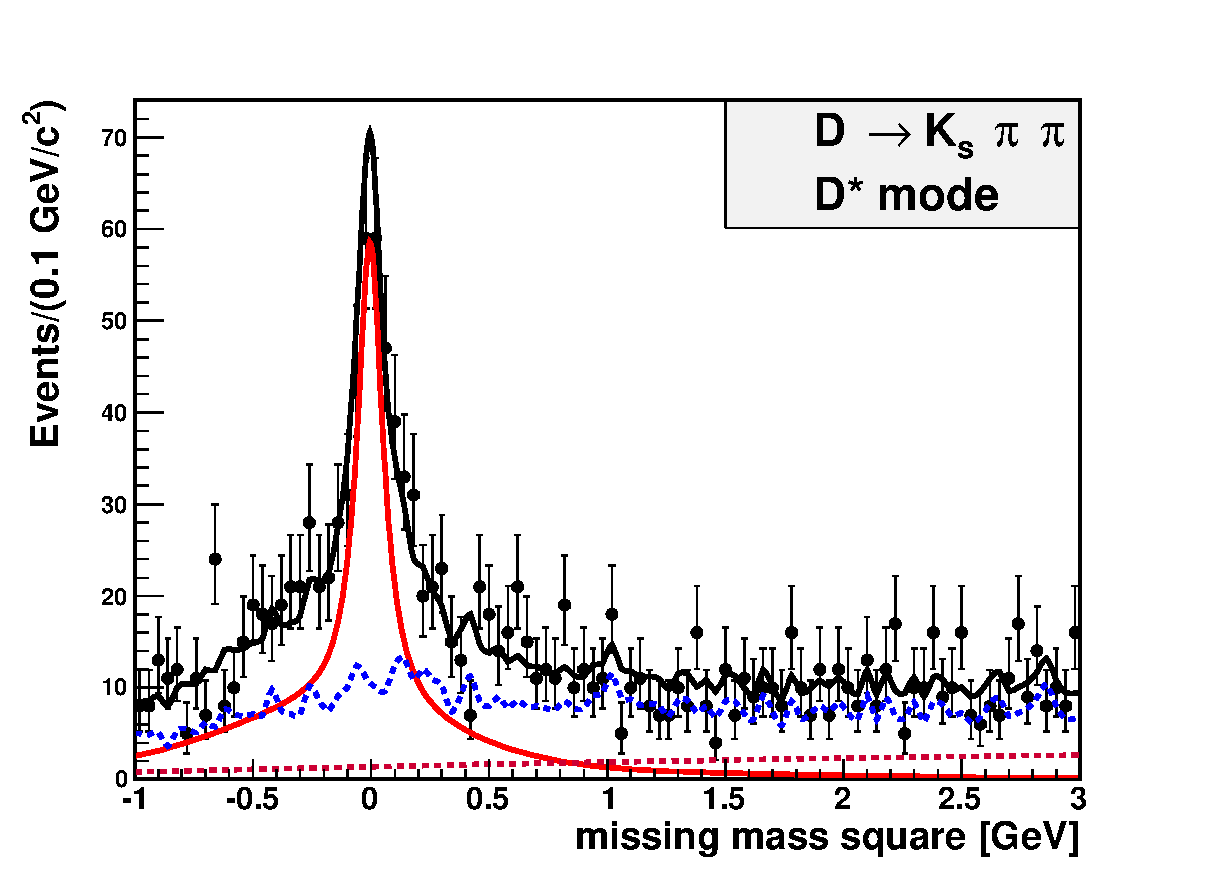
\includegraphics[width=0.3\textwidth]{Controlsample_figure/eecl_v2_0428_mbc_6_v2.eps}
		\label{condatafitdsks2pi}
	}
    	\subfigure[$B^0 \rightarrow D^{-}(K_s \pi) \ell \nu$]{
		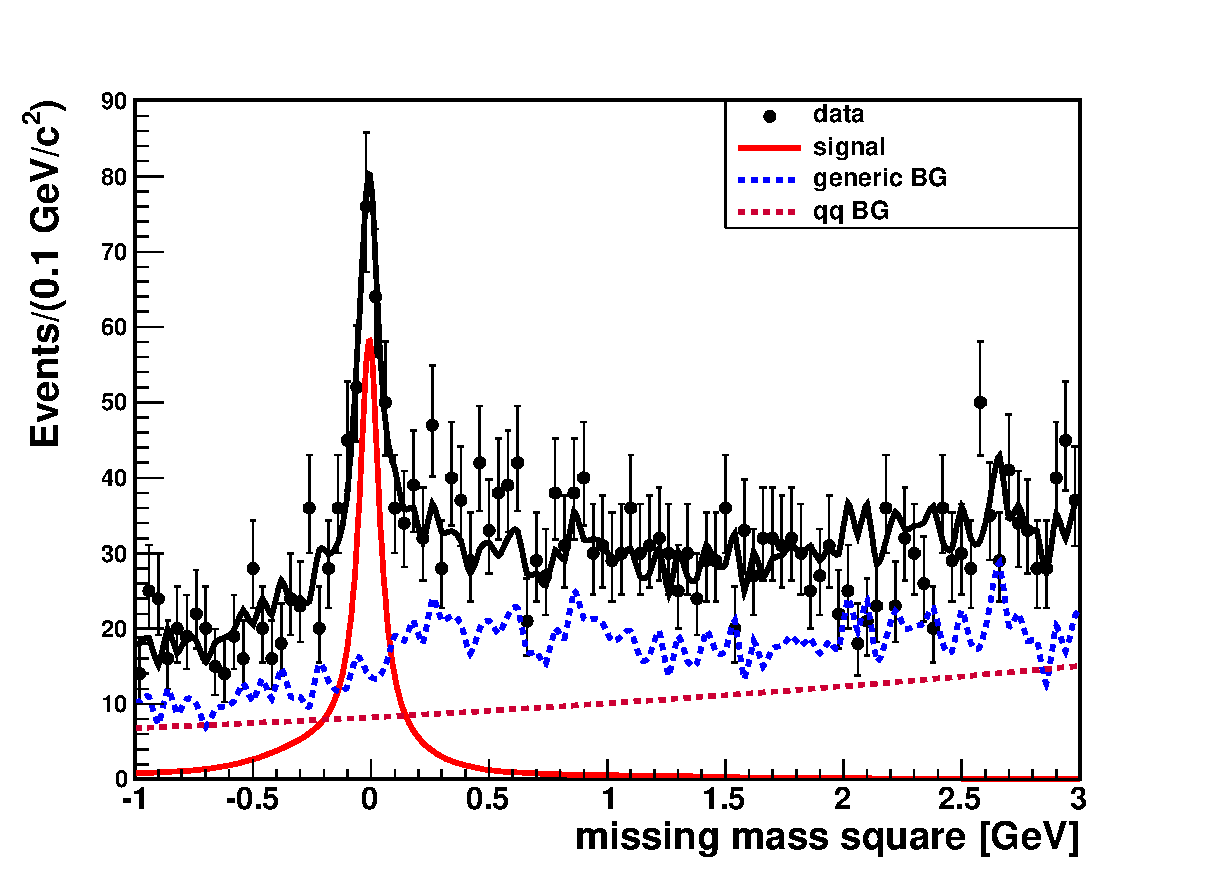
\includegraphics[width=0.45\textwidth]{Controlsample_figure/missingmass_fit_data.eps}
		\label{condatafit0dkspi}
	}
    	\subfigure[$B^0 \rightarrow D^{-}(K 2 \pi) \ell \nu$]{
		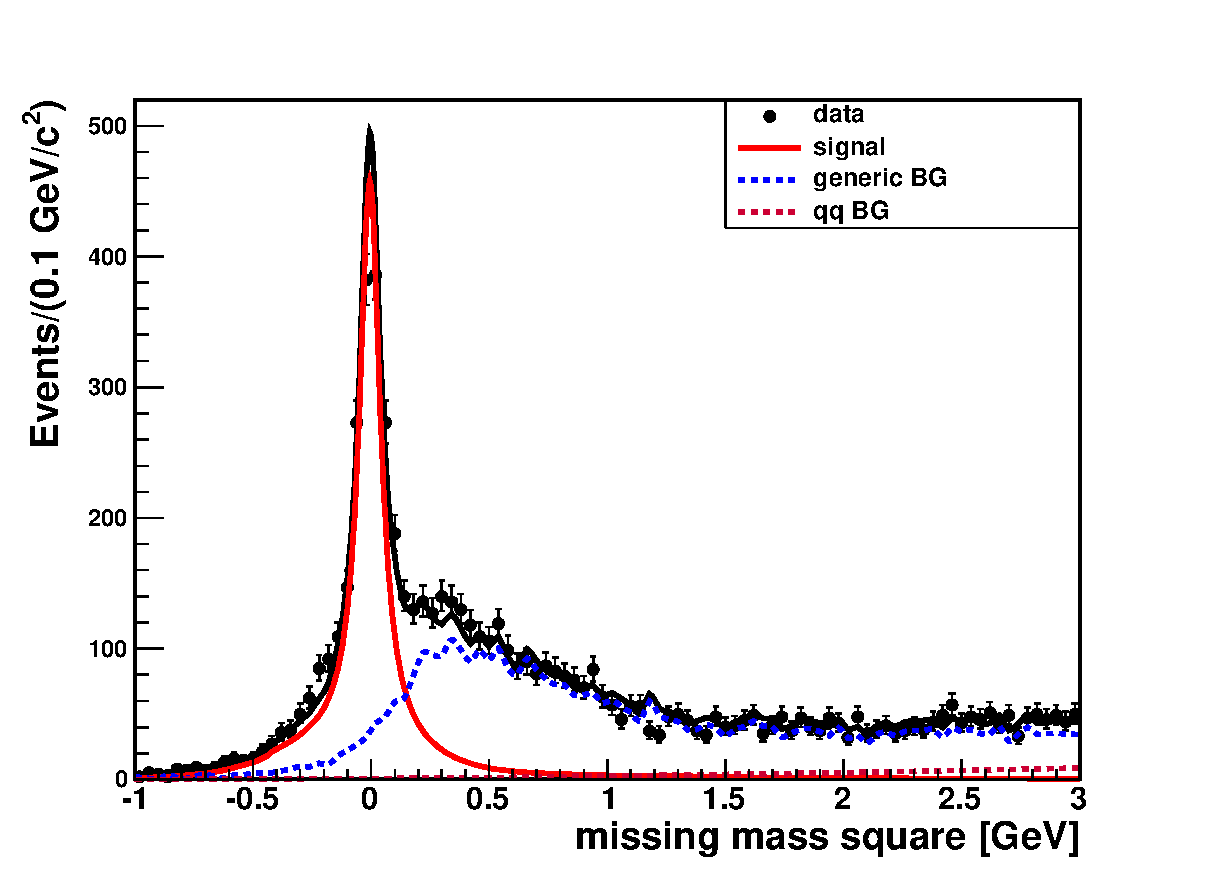
\includegraphics[width=0.45\textwidth]{Controlsample_figure/missingmass_fit_datakpipi.eps}
		\label{condatafit0dk2pi}
	}
	\caption{Data fit result for all $B \rightarrow D \ell \nu$, red solid line is signal PDF, blue dash line is generic PDF, pink dash line is continuum PDF, black dot with error is data point.}
    	\label{condatafit}	
\end{figure}
\begin{table}[h]
\small
\begin{center}
\begin{tabular}{ |p{3.7cm}||p{2cm}||p{2cm}||p{2.4cm}||p{2.4cm}| }
\hline
 Mode & $N_{yield}$ & Efficiency & $\mathcal{B}$ measurement & PDG value  \\
 \hline
 $ B^+ \rightarrow D^0(K\pi) \ell \nu$ & $3240.8^{+84.6}_{-83.5}$  & $9.77 \times 10^{-3}$ &1.90 $\pm$ 0.06 & $2.27 \pm 0.11$ \\ 
  \hline
 $ B^+ \rightarrow D^0(K 3 \pi) \ell \nu$ & $3251.4^{+101.7}_{-100.8}$ & $8.91 \times 10^{-3}$ &2.14 $\pm$ 0.07 & $2.27 \pm 0.11$ \\ 
  \hline
 $ B^+ \rightarrow D^0(K_s 2 \pi) \ell \nu$ &$1095.5^{+87.7}_{-86.6}$ & $3.03 \times 10^{-3}$ &2.02 $\pm$ 0.07 & $2.27 \pm 0.11$ \\ 
  \hline
 $ B^+ \rightarrow D^{*0}(K\pi) \ell \nu$ &$1757.5^{+54.6}_{-53.9}$ & $5.51 \times 10^{-3}$&4.58 $\pm$ 0.17 & $5.69 \pm 0.19$ \\ 
  \hline
 $ B^+ \rightarrow D^{*0}(K 3 \pi) \ell \nu$ &$1687.2^{+64.8}_{-63.6}$ & $4.49 \times 10^{-3}$ &5.52 $\pm$ 0.21 & $5.69 \pm 0.19$ \\ 
  \hline
 $ B^+ \rightarrow D^{*0}(K_s 2 \pi) \ell \nu$ &$508.2^{+47.5}_{-46.1}$ & $1.59 \times 10^{-3}$ &4.49 $\pm$ 0.05 & $5.69 \pm 0.19$ \\ 
  \hline
 $ B^0 \rightarrow D^-(K_s\pi) \ell \nu$ &$318.6^{+29.7}_{-28.7}$ & $1.48 \times 10^{-3}$ &1.37 $\pm$ 0.12 & $2.19 \pm 0.12$ \\ 
  \hline
 $ B^0 \rightarrow D^-(K 2 \pi) \ell \nu$ &$2316.2^{+59.1}_{-58.2}$ & $1.81 \times 10^{-3}$ &1.26 $\pm$ 0.03 & $2.19 \pm 0.12$ \\ 
 \hline
 \hline
\end{tabular}
\caption{The measurement result and efficiency.} \label{t:brbeforec}
\end{center}
\end{table}
\begin{table}[h]
\small
\begin{center}
\begin{tabular}{ |p{3.7cm}||p{2cm}||p{2cm}||p{2.4cm}||p{2.4cm}| }
\hline
 Mode & $\mathcal{C}_{tag}$ & $\mathcal{C}_{PID}$ & $\mathcal{B}$ measurement & PDG value  \\
 \hline
 $ B^+ \rightarrow D^0(K\pi) \ell \nu$ &0.8453  & 0.9711 &2.32 $\pm$ 0.06 & $2.27 \pm 0.11$ \\ 
  \hline
 $ B^+ \rightarrow D^0(K 3 \pi) \ell \nu$ &0.9961  & 0.9293 &2.31 $\pm$ 0.07 & $2.27 \pm 0.11$ \\ 
  \hline
 $ B^+ \rightarrow D^0(K_s 2 \pi) \ell \nu$ &0.9560  & 0.8618 &2.45 $\pm$ 0.21 & $2.27 \pm 0.11$ \\ 
  \hline
 $ B^+ \rightarrow D^{*0}(K\pi) \ell \nu$ &0.8793  & 0.9317 &5.59 $\pm$ 0.17 & $5.69 \pm 0.19$ \\ 
  \hline
 $ B^+ \rightarrow D^{*0}(K 3 \pi) \ell \nu$ &1.0751  & 0.9187 &5.59 $\pm$ 0.21 & $5.69 \pm 0.19$ \\ 
  \hline
 $ B^+ \rightarrow D^{*0}(K_s 2 \pi) \ell \nu$ &0.8933  & 0.9531 &5.27 $\pm$ 0.05 & $5.69 \pm 0.19$ \\ 
  \hline
 $ B^0 \rightarrow D^-(K_s\pi) \ell \nu$ &0.6584  & 0.8948 &2.33 $\pm$ 0.12 & $2.19 \pm 0.12$ \\ 
  \hline
 $ B^0 \rightarrow D^-(K 2 \pi) \ell \nu$ &0.6507  & 0.9386 &2.07 $\pm$ 0.03 & $2.19 \pm 0.12$ \\ 
 \hline
 \hline
\end{tabular}
\caption{The measurement result with calibration.} \label{t:brafterc}
\end{center}
\end{table}
\subsection{Branching Ratio Calibration}
The measured $\mathcal{B}$ for all channel are not consist with PDG value yet, it because the discrepancy between MC sample and real data, we find out the dominate factor of the discrepancy is from  Fullrecon module, because the main hadronic decay channels are not precisely measure, resulting in the tag-side efficiency distortion. The other factor contribute to the MC-data discrepancy is PID selection.the efficiencies factorize become:
\begin{equation}
\label{eq:efficiencycorrect}
\mathcal{E}_{corrected} = \mathcal{E}_{sig} \times \mathcal{E}_{tag} \times \mathcal{C}_{tag} \times \mathcal{C}_{PID}
\end{equation}
We determine the $\mathcal{C}_{tag}$ by follow the method which is done by the CKM group \cite{ref:Varvell2012}, they check the MC-data discrepancy tag mode by tag mode and also involve an integral over the distribution of the NeuroBayes output variable ln$NB_{out}$. For the $\mathcal{C}_{PID}$ calculation, we use the formula:
\begin{equation}
\label{eq:efficiencycorrect}
\mathcal{C}_{PID} = \mathcal{C}_{KID} \times \mathcal{C}_{\pi ID} \times \mathcal{C}_{\ell ~ ID} = \frac{\epsilon_{K,data}}{\epsilon_{K,MC}} \times \frac{\epsilon_{\pi,data}}{\epsilon_{\pi,MC}} \times \frac{\epsilon_{\ell,data}}{\epsilon_{\ell,MC}}
\end{equation}
and, 
\begin{equation}
\label{eq:edefinite}
\epsilon = \frac{N_{\rm{with ~ PID ~ selection}}}{\rm{N_{without ~ PID ~ selection}}}
\end{equation}
The $\mathcal{C}_{tag}$, $\mathcal{C}_{PID}$ and the corrected measure branching ratio for all control sample channels are shown in table  \ref{t:brafterc}. The Branching ratio measure result after Fullrecon and PID calibration are all consistent with PDG value.

\section{Systematic Uncertainties}
Several systematic uncertainties are discussed in the section. The systematic errors are categorized into two part, one are bin independent systematic errors, there are $N_{BB}$, PID, track, tag efficiency and veto study. The other is bin dependent systematic errors, i.e. Neurobayes. The summary of bin independent systematic error are shown in table \ref{t:sysid}, and the summary of the bin dependent Neurobayes systematic errors are shown in table \ref{t:sysd}. The summation of the systematic error include bin-by-bin Neurobayes systematic error are shown in table \ref{t:sysall} In the following subsection, we'll discuss in detail for those systematic uncertainties. 
\begin{table}[h]
\begin{center} 
\begin{tabu}to \textwidth{ |X[l]|X[c]|X[c]|X[c]|X[c]|X[c]| }
\hline
Source & $K^+$ & $K^{*+}(K^+ \pi^0)$ & $K^{*+}(K_s \pi^+)$ & $K^{*0}$ & $K_s$\\ 
\hline
$N_{BB}$ & 1.4\% & 1.4\% & 1.4\% &1.4\% & 1.4\%\\
\hline
Track & 0.35\% & 0.35\% & 0.35\% &0.7\% & - \\
\hline
K/$\pi$ PID & 0.83\% & 0.91\% & 0.96\% &1.3\% & - \\
\hline
Track veto & 0.75\% & 0.75\% & 0.75\% &0.46\% & 0.46\% \\
\hline
$K_s$ veto & 1.9\% & 1.9\% & 1.9\% &2.4\% & 2.4\% \\
\hline
Tag efficiency & 4.2\% & 4.2\% & 4.2\% &4.5\% & 4.5\% \\
\hline
$K_s$ & - & - & 2.23\% & - & 2.23\% \\
\hline
$\pi^0$ & - & 3\% & - & - & - \\
\hline
sum & 4.96\% & 5.81\% & 5.46\% & 5.51\% & 5.76\% \\
\hline
\end{tabu}
\caption{The summary of bin independent systematic errors.} \label{t:sysd}
\end{center}
\end{table}

\begin{table}[h]
\begin{center}
\begin{tabu}to \textwidth{ |X[l]|X[c]|X[c]|X[c]|X[c]|X[c]| }
\hline
Source & $K^+$ & $K^{*+}(K^+ \pi^0)$ & $K^{*+}(K_s \pi^+)$ & $K^{*0}$ & $K_s$\\ 
\hline
bin1 & 5.27\% & 7.19\% & 2.81\% &0.12\% & 1.58\%\\
\hline
bin2 & 2.35\% & 5.21\% & 3.19\% &0.09\% & 3.57\% \\
\hline
bin3 & 6.62\% & 5.04\% & 5.13\% &7.78\% & 3.85\% \\
\hline
bin4 & 8.01\% & 5.20\% & 5.38\% &0.89\% & 1.72\% \\
\hline
bin5 & 7.49\% & 6.38\% & 10.0\% &12.39\% & 3.74\% \\
\hline
bin6 & 8.18\% & 1.64\% & 10.2\% &1.03\% & 2.78\% \\
\hline
bin7 & 6.25\% & 6.38\% & 0.18\% & 1.03\% & 0.93\% \\
\hline
bin8 & 7.49\% & - & - & - & - \\
\hline
bin9 & 3.59\% & - & - & - & - \\
\hline
\end{tabu}
\caption{The summary of bin dependent Neurobayes systematic errors.} \label{t:sysid}
\end{center}
\end{table}

\begin{table}[h]
\begin{center}
\begin{tabu}to \textwidth{ |X[l]|X[c]|X[c]|X[c]|X[c]|X[c]| }
\hline
Source & $K^+$ & $K^{*+}(K^+ \pi^0)$ & $K^{*+}(K_s \pi^+)$ & $K^{*0}$ & $K_s$\\ 
\hline
bin1 & 7.24\% & 9.24\% & 6.14\% &5.51\% & 5.92\%\\
\hline
bin2 & 5.49\% & 7.80\% & 6.32\% &5.51\% & 6.78\% \\
\hline
bin3 & 8.27\% & 7.69\% & 7.49\% &9.53\% & 6.93\% \\
\hline
bin4 & 9.42\% & 7.80\% & 7.67\% &5.58\% & 6.01\% \\
\hline
bin5 & 8.98\% & 8.63\% & 11.39\% &13.56\% & 6.87\% \\
\hline
bin6 & 9.57\% & 6.04\% & 11.57\% &5.61\% & 6.40\% \\
\hline
bin7 & 7.98\% & 8.63\% & 5.46\% & 5.61\% & 5.77\% \\
\hline
bin8 & 8.98\% & - & - & - & - \\
\hline
bin9 & 6.12\% & - & - & - & - \\
\hline
\end{tabu}
\caption{The summation of the systematic error for each bin and mode, the result include Neurobayes systematic uncertainty} \label{t:sysall}
\end{center}
\end{table}


\subsection{Number of $B\bar{B}$}
The number of $B\bar{B}$ pairs for experiment 7 to 65 is 771.581$\pm$10.566$\times 10^6$. The systematic error on $B\bar{B}$ is 1.4\%.
\subsection{Tracking uncertainty}
Tracking reconstruction of charged particles are studies by using partially reconstructed $D^{*+} \rightarrow D^0(\pi^+\pi^-\pi^0)\pi^+$ decay sample, with the $P_T > 200 $ MeV/c. The systematic uncertainty of the charge tracks are estimated to be $(-0.13 \pm 0.30 \pm 0.10 \%)$ for each track. We apply the systematic error to be 0.35 \% per track in this study.
\subsection{K/$\pi$ PID uncertainty}
The PID efficiency and fake rate are studied by using the inclusive $D^*$ sample via PID group. The K/$\pi$ efficiency and fake rate are all obtain from the official table with corresponding $P_{lab}$ and cos$\theta$.
\subsection{Tag efficiency uncertainty}
The Tag efficiency uncertainty are studied by using the method which is provide by CKM group\cite{ref:Varvell2012} ]. They use the $B\rightarrow D \ell \nu$ sample to estimate the total uncertainty of the tag bias correction for $B^+$ to be 4.2\% and for $B^0$ 4.5\%.
\subsection{$K_s$ and $\pi^0$ reconstruction uncertainty}
The overall systematic error on the $K_s$ reconstruction efficiency is estimate in \cite{ref:White2011} to be 2.23\%. The systematic error on the $\pi^0$ reconstruction efficiency is 3\% \cite{ref:Chang2012a}.
\subsection{Neurobayes systematic uncertainty}
We estimate the Neurobayes systematic uncertainty by compare the MC/data in ratio of with NB selection and without NB selection by the control sample $B \rightarrow D \ell \nu $. The MC and data yield with NB selection and without NB selection yield are obtain by fitting on missing mass square. We do the bin-by-bin estimation because we perform the different NB cut on different bin. 
